\documentclass[onecolumn]{article}
\usepackage{array,booktabs,bytefield}
\usepackage{graphicx, here}
\begin{document}

\pagenumbering{roman}

\title{Enhancement of ALSA firewire stack}
\author{Takashi Sakamoto}
\date{2014/07/23}
\maketitle{}

\begin{abstract}

Many sound devices connected to IEEE 1394 bus have been produced since 2000. To support these devices, ALSA, Linux sound subsystem, has firewire driver stack in kernel-land. But this stack supports just a few devices because of a restriction to transfer outgoing packets with PCM samples only. This is not enough for most of devices for music production because these devices require drivers to handle incoming packets for timestamp synchronization, multiplex/demultiplex different types of data to the same packet. Instead of ALSA, FFADO, a project to develop user-land driver, supports many devices. But there is no way for ALSA applications to use FFADO directly. In 2014, ALSA firewire stack is enhanced with new drivers to support around 80 devices, to enable ALSA applications to communicate the devices directly. This enhancement was pulled into Linux 3.16.

\end{abstract}

\section*{Acknowledgement}

I would like to appreciate many people who help me for this work, especially two developers and three dedicated testers. Clemens Ladisch is a maintainer of ALSA firewire stack. Without his work for this stack and original Fireworks driver, I might have no interest in this category of devices. Moreover, without his comments and reviews, my patches were not merged into ALSA upstream. Daniel Wagner is a founder of former FreeBoB project. Without his help, I cannot access BeBoB related resources and have no opportunity to understand BeBoB functionalities. Darren Anderson, Maximilian Engelhardt and David Henningsson patiently tested my drivers with some models which they have. Without their continuous and feasible feedbacks, I might have no confidence for my drivers.

\newpage

\tableofcontents

\newpage

\pagenumbering{arabic}

\section{Introduction}

Linux is an operating system widely used on various platform, and its sound subsystem, Advanced Linux Sound Architecture (ALSA) is used on several platforms. On PC/AT-compatible platform, there are people who have enthusiasms to use Linux for music production. They require sound devices with unique functionality such like internal mixing and synchronization. Some of them (not all of them) prefer to sound devices connected to IEEE 1394 bus because the devices satisfy their requirement.

But ALSA, itself, has a weak stack to handle the devices. Instead of ALSA, user-land driver satisfies the users. A project to develop the driver is FFADO. FFADO gives a library for applications. This library includes Application Programming Interface (API) to communicate to the devices. Although there are much ALSA applications, there are less FFADO applications. And there's no way for ALSA applications to use FFADO directly. This means that ALSA applications don't handle most of the sound devices directly.

I\footnote{Author} realized this issue in 2009. After investigating, I concluded that enhancement of ALSA firewire stack is a better solution. I write this report to explain the conclusion and my work for this stack.

In this report, at first, I review some specifications related to the devices. Next, I describe devices' features. Then I investigate software implementation in user-land and in kernel-land to seek solution. Finally, I explain my work for ALSA firewire stack.


\section{Common Specifications}

The sound devices connected to IEEE 1394 bus use IEC 61883-1/6 for its communication protocol. The main feature of this protocol is packet transmittion for audio and music data. In this section, I review IEEE 1394, IEEE 1212, IEC 61883-1/6, AV/C command and OHCI 1394 to help understanding of devices' features. This report is not for explanations of specifications, thus I pick up information needed to implement software drivers.

\subsection{IEEE 1394 bus}

IEEE 1394 is a serial bus. IEEE published its first standard documents in 1995\cite{ieee1394-1}. Between 2000 and 2006, some supplements were added\cite{ieee1394-1-a, ieee1394-1-b, ieee1394-1-c}. And in 2008, it was updated\cite{ieee1394-2}.

IEEE 1394 bus consists of Physical layer, Link layer, Transaction layer and Serial bus management. Two types of communication are available on the bus, isochronous and asynchronous.

\subsubsection{Physical layer}
IEEE 1394 Physical layer defines two types of environment, cable and backplane, however I've never seen the backplane environment. I describe about cable environment. In cable environment, a unique cable and connectors are defined. In this environment, any bus topologies such like tree and star are available. A half duplex communication with arbitration is used. For the communication, analog signal is used for the arbitration. After the arbitration, encoded signal is used for digital data.


\subsubsection{Link layer}
IEEE 1394 Link layer defines the way to control isochronous cycle, to receive or transmit packets, to fragment a packet.


\subsubsection{Transaction layer}
IEEE 1394 Transaction layer defines the way to control nodes over the same bus. This layer uses IEEE 1212 for addressing of nodes and the types of transaction.

\subsubsection{Serial bus management}
IEEE 1394 Serial bus management defines the way to manage bus topology, transmission and resources for isochronous communication. This layer works with the other layers.

\subsubsection{Isochronous communication}
IEEE 1394 isochronous communication guarantees to transfer packets at 8,000 times per second (8.0kHz). One cycle master broadcasts cycle start packets to start a communication, then the other nodes transfer packet with a certain channel. This channel is express within 6bit field of an isochronous packet. Receivers deal with packets identified by the channel.

\begin{figure}[H]
\centering
\begin{bytefield}[bitwidth=auto,endianness=big]{32}
	\bitheader{0-31} \\
	\begin{rightwordgroup}{packet \\ header}
		\bitbox{16}{data length} &
		\bitbox{2}{tag} &
		\bitbox{6}{channel} &
		\bitbox{4}{tcode} &
		\bitbox{4}{sy} \\
		\wordbox{1}{header CRC}
	\end{rightwordgroup} \\
	\begin{rightwordgroup}{packet payload}
		\wordbox[tlr]{3}{data field} \\
		\bitbox[blr]{16}{} &
		\bitbox{16}{zero pad bytes (if necessary)} \\
		\wordbox{1}{payload CRC}
	\end{rightwordgroup}
\end{bytefield}
\caption{Isochronous packet structure}
\label{fig:iso-packet}
\end{figure}

In Figure \ref{fig:iso-packet}, data length: the length of data field, tag: the packet format, channel: the channel number for this packet, tcode: the data format of isochronous packet, sy: application specific control field.

The value of tcode field is usually b1010, the value of tag field is usually b01 for Common Isochronous Packet(CIP)\cite{iec61883-1-3}, 

\subsubsection{Asynchronous communication}
IEEE 1394 asynchronous communication has no guarantees for delay. The packet can be fragmented. IEEE 1394 transaction layer handles this types of communication. There are two types of transaction, quadlet and block.

\begin{figure}[H]
\centering
\begin{bytefield}[bitwidth=auto,endianness=big]{32}
	\bitheader{0-31} \\
	\begin{rightwordgroup}{packet \\ header}
		\bitbox{16}{destination ID} &
		\bitbox{6}{tl} &
		\bitbox{2}{rt} &
		\bitbox{4}{\tiny tcode \\ 0000} &
		\bitbox{4}{pri} \\
		\bitbox{16}{source ID} &
		\bitbox[tlr]{16}{destination offset} \\
		\wordbox[blr]{1}{} \\
		\wordbox{1}{quadlet data} \\
		\wordbox{1}{header CRC}
	\end{rightwordgroup} \\
\end{bytefield}
\caption{Asynchronous packet structure for quadlet transaction}
\label{fig:async-packet-quadlet}
\end{figure}

\begin{figure}[H]
\centering
\begin{bytefield}[bitwidth=auto,endianness=big]{32}
	\bitheader{0-31} \\
	\begin{rightwordgroup}{packet \\ header}
		\bitbox{16}{destination ID} &
		\bitbox{6}{tl} &
		\bitbox{2}{rt} &
		\bitbox{4}{\tiny tcode \\ 0001} &
		\bitbox{4}{pri} \\
		\bitbox{16}{source ID} &
		\bitbox[tlr]{16}{destination offset} \\
		\wordbox[blr]{1}{} \\
		\bitbox{16}{data length} &
		\bitbox{16}{extended code} \\
		\wordbox{1}{header CRC} 
	\end{rightwordgroup} \\
	\begin{rightwordgroup}{payload}
		\wordbox[tlr]{3}{block data} \\
		\bitbox[blr]{16}{} &
		\bitbox{16}{zero pad bytes (if necessary)} \\
		\wordbox{1}{payload CRC}
	\end{rightwordgroup}
\end{bytefield}
\caption{Asynchronous packet structure for block transaction}
\label{fig:async-packet-block}
\end{figure}

In Figure \ref{fig:async-packet-quadlet} and \ref{fig:async-packet-block}, destination ID: node ID of destination, tl: transaction label for a pair of request and response, rt: the way to retry, tcode: the type of transaction, read/write/lock and quadlet/block and request/response, pri: priority, source ID: node ID of source, destination offset: an address offset on destination's area, data length: the length of byte of block data, extended code: the type of lock transaction.

\subsection{IEEE 1212}

IEEE 1212 is a specification for logical address space of each devices and types of transaction. The first edition was published in 1991\cite{ieee1212-1} and this was standardized in ISO/IEC 13213\cite{iso13213}. The second edition was published in 2001\cite{ieee1212-2} and supervised previous edition.

IEEE 1212 defines some entities on the bus. They are module, node and unit. The module includes some nodes and the node includes some units. The node is addressed with 64-bit width value. The node can communicate each other by transactions with the address. IEEE 1212 defines three types of transaction. They are read, write and lock transactions. The address space of each node includes Control and Status Registers (CSR) to control the state of node. The address space also includes Configuration ROM to show information of the node and unit.


\subsection{IEC 61883-1}

IEC 61883-1 defines a transmission protocol for audio-visual data and control commands which provides for the interconnection of digital audio and video equipment. The first edition was published in 1998\cite{iec61883-1-1}. The second edition was published in 2003\cite{iec61883-1-2}. The third edition supervised previous editions in 2008\cite{iec61883-1-3}.

IEC 61883-1 describes Real time data transmission protocol over IEEE 1394 bus, and Common Isochronous Packet (CIP) for a basic format of data in payload of IEEE 1394 isochronous packet. The detail of CIP is described in next subsection.

This data transmission is controlled with an idea of 'connection'. The connections is expressed in Plug Control Register (PCR). Master Plug Register (MPR) has basic information for PCRs. Both of MPR/PCR have 32bit register. The space for them is from 0xFFFF'F000'0900 to 0xFFFF'F000'09FC. A first half of this area is for output plugs and the rest is for input plugs. The first 32bit register of each area is for MPR.

The connection is controlled by Connection Management Procedure (CMP). In CMP, some fields in PCR can be changed by lock transaction to establish/break connections.

The functionality on each node can be controlled by Function Control Protocol (FCP). FCP consists of a pair of transaction for command and response. The address for command is 0xFFFF'F000'0B00 and the address for response is 0xFFFF'F000'0D00. The length of data for each transaction is limited by 512 bytes.


\subsection{IEC 61883-6}

IEC 61883-6 is a variation of IEC 61883-1 for audio and music data, so-called as AMDTP. The first edition was published in 2002\cite{iec61883-6-1}. The second edition was published in 2005 with many extensions\cite{iec61883-6-2}.

IEC 61883-1\cite{iec61883-1-1, iec61883-1-2, iec61883-1-3} allows any variations for CIP structure. The CIP header consists of some 32bit fields. The first bit in MSB means End-of-CIP-header (EOH). This bit stands when the 32bit fields is the last CIP header. The second bit in MSB is Form. This bit means the format of followed fields but the specification includes ambiguity of its meaning. In AMDTP, two quadlets CIP header with SYT field is used. I show CIP structure for AMDTP in Figure \ref{fig:amdtp-cip}. Minor fields are filled with zero.

\begin{figure}[H]
\centering
\begin{bytefield}[bitwidth=auto,endianness=big]{32}
	\bitheader{0-31} \\
	\begin{rightwordgroup}{CIP header \\ with SYT field}
		\bitbox{1}{0} &
		\bitbox{1}{0} &
		\bitbox{6}{SID} &
		\bitbox{8}{DBS} &
		\bitbox{2}{00} &
		\bitbox{3}{000} &
		\bitbox{1}{0} &
		\bitbox{2}{000} &
		\bitbox{8}{DBC} \\
		\bitbox{1}{1} &
		\bitbox{1}{0} &
		\bitbox{6}{FMT} &
		\bitbox{8}{FDF} &
		\bitbox{16}{SYT}
	\end{rightwordgroup} \\
	\begin{rightwordgroup}{data block \\ = event 1}
		\wordbox[tlr]{1}{data} \\
		\wordbox[blr]{1}{$\cdots$}
	\end{rightwordgroup} \\
	\begin{rightwordgroup}{data block \\ = event 2}
		\wordbox[tlr]{1}{data} \\
		\wordbox[blr]{1}{$\cdots$}
	\end{rightwordgroup} \\
	\wordbox{1}{$\cdots$} \\
\end{bytefield}
\caption{CIP variation for AMDTP}
\label{fig:amdtp-cip}
\end{figure}

In Figure \ref{fig:amdtp-cip}, SID: the node ID of transmitter, DBS: the number of quadlets for data blocks, DBC: the number of data blocks which has already transferred, FMT: format ID, FDF: format dependent field, SYT: the offset from isochronous cycle timer.

The value of DBC field is used to detect packet lost. In AMDTP, the value of FMT is 0x10. FDF field consists of 'Event Type' field and 'Sampling Frequency Code' field described later. On the other hand, 0xff in FDF field is No data code to indicate packet without any data. In AMDTP, the value of SYT field is used to show 'presentation time'. In detail, Section \ref{sec:clock-recovery} to page \pageref{sec:clock-recovery}.

After CIP headers, some data blocks follows. In AMDTP, one data block represents an event. IEC 61883-6\cite{iec61883-6-1, iec61883-6-2} doesn't define the meaning of event, although the event may be a batch of data accompanied with the same timing. There are some ways to describe the data. AM824 is mostly used.

AM824 represents data by 32bit field that has an 8bit label and 24bit data field. In IEC 61883-6:2002\cite{iec61883-6-1}, AM824 can describe three types of data, IEC 60958 Conformant, Raw Audio and MIDI Conformant. In IEC 61883-6:2005\cite{iec61883-6-2}, Raw Audio is renamed as Multi Bit Linear Audio (MBLA) and some data types are newly supported.

The event is for audio and music, therefore AMDTP is dominated by sampling frequency. FDF field of CIP header indicates the sampling frequency and the type of event. The 4bit in the most significant bit is EVT field to show the way to describe the data of event, and the lower 3bit of 4bit in the least significant bit is SFC to show nominal sampling frequency. The rest 1bit is N-flag. This flag is used to show the mode of rate control. When this flag does not stand, it means clock based rate control, described in Section \ref{sec:clock-recovery} to page \pageref{sec:clock-recovery}. When the flag stands, it means command based rate control\cite{iec61883-6-2, avc-rate-control}. For AM824, the value of EVT field is b0000. The values of SFC field is shown at Table \ref{tbl:sfc-fdf}. For most of sound devices, N-flag doesn't stand.

\begin{figure}[H]
\centering
\begin{bytefield}[bitwidth=auto,endianness=big]{8}
	\bitheader{0-7} \\
	\bitbox{4}{EVT} &
	\bitbox{1}{N} &
	\bitbox{3}{SFC} &
\end{bytefield}
\caption{FDF field for AMDTP}
\label{amdtp-fdf}
\end{figure}

\begin{table}[H]
	\centering
	\caption{{The value of SFC field in FDF field}}
	\label{tbl:sfc-fdf}
	\begin{tabular}{ccc} \toprule
		Nominal Sampling Frequency & SFC \\ \midrule
		32.0	& b000 \\
		44.1	& b001 \\
		48.0	& b010 \\
		88.2	& b011 \\
		96.0	& b100 \\
		176.4	& b101 \\
		192.0	& b110 \\ \bottomrule
	\end{tabular}
\end{table}

For detail of the way to transfer packets, see Section \ref{sec:clock-recovery} to page \pageref{sec:clock-recovery}.

\subsection{AV/C commands}

IEC 61883 series came from documents which 1394 Trade Association (1394TA) published. Especially, actual application of FCP is in 1394TA documents and not in any public documents. In 1394TA documents, the application is called as 'AV/C commands'. There are much variations of AV/C command, including over-specifications. A part of documents are applied to the sound devices\cite{avc-general-4-2, avc-audio-1, avc-connection-1, avc-music-1, avc-descriptor-1, avc-info-block-1, avc-general-enhancement, avc-stream-format-1, avc-stream-format-1-1, avc-rate-control}.

\subsection{1394 Open Host Controller Interface}
\label{ohci-1394}

1394 Open Host Controller Interface (OHCI 1394) is an implementation of the link layer protocol of IEEE 1394, with additional features to support the transaction and bus management layers. This specification uses Direct Media Access (DMA) engines for high-performance data transfer and a host bus interface. The first edition was published in 1997\cite{ohci1394-1} and revised in 2000\cite{ohci1394-1-1}.

OHCI 1394 describes software interface with register, interrupt and DMA. For PC/AT-compatible platform, OHCI 1394 is implemented as card devices on PCI/PCI-Express bus.

OHCI 1394 represents both of asynchronous and isochronous communication as context, which includes a list of descriptor. A descriptor includes information of a packet for each communication. The information includes an address for DMA buffer. The data in the address is transferred between system and controller device by DMA. After transferring, interrupts are generated according to information in the descriptor. The minimum number of isochronous context is 4 and the maximum is 32, for one direction.

\section{Device features}

The sound devices for music production have unique features. In this section, I describe such features to consider software implementation.

\subsection{Clock recovery}
\label{sec:clock-recovery}

Clock recovery is a mechanism for receivers to regenerate transmitter's clock cycle.

In IEEE 1394\cite{ieee1394-2}, isochronous-capable nodes should have 32bit CYCLE\_TIMER register. The low-order 12 bits of the register are a modulo 3,072 counter, which increments once every 24.576MHz (or 40.69 nano second). The next 13 higher-order bits are a count of 8.0kHz (or 125us) cycles, and the highest 7 bits count seconds.

\begin{figure}[htbp]
\centering
\begin{bytefield}[bitwidth=auto,endianness=big]{32}
	\bitheader{0-31} \\
	\bitbox{7}{seconds\_count} &
	\bitbox{13}{cycle\_count} &
	\bitbox{12}{cycle\_offset}
\end{bytefield}
\caption{{CYCLE\_TIMER register}}
\label{cycle_timer}
\end{figure}

In usual implementation, the register count up according to 24.576MHz clock given by IEEE 1394 Link layer chipset.

When the cycle\_offset field rolls over, cycle master node broadcasts a cycle-start packet after arbitration. This packet has a cycle\_time field. The cycle\_time field includes the value of CYCLE\_TIMER register. After receiving cycle-start packet, transmitters and receivers update their CYCLE\_TIMER register with the value. As a result, the transmitters and receivers can maintain local time reference to cycle master. Then transmitters start arbitration and transmit an isochronous packet with a certain channel and the receivers receive isochronous packet with a favorite channel. Actual intervals between the cycle-start packets are different depending on bandwidth usage, see Figure \ref{fig:cycle-start}.

\begin{figure}[htbp]
\centering

\includegraphics[scale=0.75]{./img/cycle-start-packet.svg.eps}
\caption{{cycle-start packet and nominal isochronous cycle}}
\label{fig:cycle-start}
\end{figure}

IEC 61883-1 defines SYT field in CIP header (see Figure \ref{fig:amdtp-cip} to page \pageref{fig:amdtp-cip}). In IEC 61883-6, this field is used to calculate 'presentation time'. The 'presentation time' represents the timestamp for a certain event in a packet. The transmitter calculates offset for the timing of sampling clock from local isochronous cycle reference, then transfers the value in SYT field of a packet. The receivers calculate 'presentation time' with the value of SYT field in the packet and local isochronous cycle reference.

One packet has one SYT field in its CIP header, while one packet can include several data blocks. All of data blocks cannot have 'presentation time'. The interval between data blocks with 'presentation time' is defined as SYT\_INTERVAL.

\begin{table}[ht]
	\centering
	\caption{{The value of SYT\_INTERVAL}}
	\label{syt_interval}
	\begin{tabular}{cc} \toprule
		Sample transmission frequency & SYT\_INTERVAL \\ \midrule
		32.0	& 8	\\
		44.1	& 8	\\
		48.0	& 8	\\
		88.2	& 16	\\
		96.0	& 16	\\
		176.4	& 32	\\
		192.0	& 32	\\ \bottomrule
	\end{tabular}
\end{table}

If there's a packet which includes no data blocks with 'presentation time', the value of SYT is 'No Information' code (0xffff). It's different to decide the data block with 'presentation time', depending on mode to transfer packets.

In IEC 61883-6\cite{iec61883-6-1,iec61883-6-2}, there are two modes to transfer packets; blocking and non-blocking. The differences between these two modes are transfer-delay and the number of data blocks which a packet can includes.

In blocking mode, the number of data blocks in an packet is fixed to the value of SYT\_INTERVAL, thus 'presentation time' is for the first data block in a packet. A transmitter must wait until all of samples in a packet are sampled, therefore the transfer delay is larger than default value by one packet.

\begin{figure}[H]
	\centering
	
\includegraphics[scale=0.6]{./img/amdtp-blocking.svg.eps}
	\caption{{AMDTP in blocking mode}}
	\label{amdtp-blocking}
\end{figure}

In non-blocking mode, a packet can include different number of data blocks. The transmitter can transfer packets according to nominal isochronous cycle without waiting for fixed numbers of event. The transfer delay equals to default value, while it's more complicated to decide which data block is accompanied by 'presentation timestamp' of a packet.

\begin{figure}[H]
	\centering
	
\includegraphics[scale=0.6]{./img/amdtp-nonblocking.svg.eps}
	\caption{{AMDTP in non-blocking mode}}
	\label{amdtp-nonblockingstart}
\end{figure}

A transmitter decides a data block with 'presentation time' in this condition:

\begin{equation}
	mod(DBC, SYT\_INTERVAL) = 0
\end{equation}

Then receivers calculates an index of data block with 'presentation timestamp' according to this formula:

\begin{equation}
	index = mod((SYT\_INTERVAL - mod(DBC, SYT\_INTERVAL)), SYT\_INTERVAL)
\end{equation}

In both modes, the receivers can generate 'synchronization clock frequency' to use the sequence of SYT field and the local time reference, according to this formula.

\begin{equation}
	Fsync = STF / SYT\_INTERVAL < 8,000
\end{equation}

Here Fsync is the synchronization clock frequency. STF is the sampling transmission frequency, equals to sampling clock frequency.

\begin{table}[H]
	\centering
	\caption{{Synchronization clock frequency at each sampling transmission frequency}}
	\label{fsync}
	\begin{tabular}{ccc} \toprule
		STF & SYT\_INTERVAL & Fsync \\ \midrule
		32.0	& 8	& 4,000 \\
		44.1	& 8	& 5,512 \\
		48.0	& 8	& 6,000 \\
		88.2	& 16	& 5,512 \\
		96.0	& 16	& 6,000 \\
		176.4	& 32	& 5,512 \\
		192.0	& 32	& 6,000 \\ \bottomrule
	\end{tabular}
\end{table}

The receivers can use the pulse of this frequency for a reference of phase lock loop (PLL) circuit. This is a mechanism of 'clock recovery'. For an example of actual implementation, see\cite{icelynx}.


\subsection{Signal processing for internal mixing}
\label{sec:internal-mixing}

Most devices for music production have several ports for analog/digital audio input/output. Such devices have DSP to process signals from/to the ports for internal mixing. This is 'zero latency hardware monitoring', which each vendor insists.

In the DSP side, outgoing packet is a sink of audio signals and incoming packet is a source of audio signals. The DSP is between IEC 61883-1/6 layer and DAC/ADC for audio ports, therefore a device generates no sound when DSP has no settings of routing between sinks and sources.

The way to control the DSP behaviour depends on each chipset or model.

\begin{figure}[H]
	\centering
	
\includegraphics{./img/dsp-route.svg.eps}
	\caption{{Signal processing between sources and sinks}}
	\label{dsp-route}
\end{figure}

\subsection{Some options for sampling clock source for DSP}

Most devices for music production have several options for source of clock. The source is used for input clock of DSP. The options are:
\begin{itemize}
	\item Signal from internal clock source
	\item Signal from input of S/PDIF, ADAT or Word Clock
	\item Signal of nominal isochronous cycle (8kHz)
	\item Signal of recovered clock as described in previous subsection (4.0/5.512/6.0kHz)
\end{itemize}

The way to change or check current source of clock depends on each device chipset. When an external source is selected, sampling rate should be fixed according to the signal from an external source.

\subsection{Duplex streams with timestamp synchronization}
\label{sec:duplex-streams}

As described in former subsection, each AMDTP packet delivers 'presentation time' in the sequence of value in SYT field. When a pair of device supports both of transmitting/receiving streams, the generator of the timestamp should be one of the devices for better synchronization between transmitter and receiver. This idea requires timing slaves to regenerate the sequence of value in SYT field for outgoing packets according to an incoming packet.

\begin{figure}[H]
	\centering
	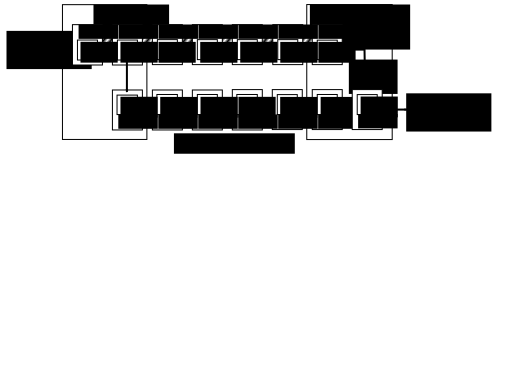
\includegraphics{./img/duplex-timestamp.svg.eps}
	\caption{{Duplex streams, timing master and slave}}
	\label{duplex-timestamp}
\end{figure}


\subsection{Different formation of data channels in a data block of packet}
\label{sec:formation-data-block}

In IEC 61883-6\cite{iec61883-6-1, iec61883-6-2}, a data block can include several types of data in each data channel. For example, MBLA data channel for PCM samples, MIDI Conformant data channel for MIDI messages and IEC 60958 Conformant data channel for PCM samples. Each model has different number of data channel and specific formation of data channels, depending on sampling frequency and a certain modes, even if these models use the same chipset.

\begin{figure}[H]
	\centering
	
\includegraphics{./img/data-block-formation.svg.eps}
	\caption{{Samples for formations of data blocks in different models with the same device chipset}}
	\label{dsp-route}
\end{figure}

For example, Model A, B, C use the same device chipset. Model A has 4 MBLA data channels at all of supported sampling rates, Model B has 8 MBLA data channels and 1 MIDI Conformant data channel at 44.1/48.0kHz, but 4 MBLA data channels and 1 MIDI Conformant data channel at 88.2/96.0kHz. Model C has the same formation at each sampling rate as Model B has, while in a certain mode Model C has 2 MBLA data channel and 1 MIDI Conformant data channel at 44.1/48.0/88.2/96.0kHz.

The way to get information about the formation depends on each chipset.

\subsection{Chipset specific operations and quirks}

Although there are some common specifications, each device has specific quirks due to chipset or vendor's customization. Especially, the way to control DSP is largely different. Currently quirks of four chipsets are clear.

\subsubsection{Fireworks}
Fireworks is a board module which Echo Audio produced. This module consists of three chipsets; Communication chipset for IEEE 1394 PHY/Link and IEC 61883-1/6 (Texas Instruments iceLynx Micro), DSP or/and FPGA for signal processing, flash Memory to store firmwares.

For transaction, fireworks uses both of AV/C commands and specific mechanism. Fireworks supports some commands in AV/C General\cite{avc-general-4-2}, AV/C Descriptor mechanism\cite{avc-general-enhancement}, while drivers can also transfer requests to a specific address on a device, and the device transfers responses to a specific address on the controller. By default, 0xecc0'0000'0000 is for requests and 0xecc0'8000'0000 is for responses. In IEEE 1212, these addresses are in "Memory space" and have no side effects against reading/writing memories. But actually Fireworks transaction has side effects according to unique request/response sets. This transaction is transferred to the addresses, while there's another way to transfer requests and responses in frame of AV/C vendor specific commands.

Fireworks manages streams by CMP and transfers AMDTP packets in blocking mode. The streams are not fully compliant to IEC 61883-1. In IEC 61883-1, the value of data block counter means the number of packets which has already transferred, while in Fireworks it means the number of data blocks in current packet. Furthermore, its empty packets are transferred at tag b00 in isochronous packet header. Additionally, Fireworks has more quirks depending on firmware version for iceLynx Micro.


\subsubsection{BeBoB}
BeBoB is 'BridgeCo enhanced Breakout Box'. This is installed to firewire devices with DM1000/DM1100/DM1500 chipset. It gives common ways for host system to handle BeBoB based devices.

BeBoB transfers AMDTP packets in blocking mode. BeBoB uses CMP to maintain AMDTP streams but some BeBoB based devices need both connections to transmit AMDTP stream.

BeBoB supports some commands in AV/C General\cite{avc-general-4-2}, AV/C Audio subunit\cite{avc-audio-1}, AV/C Music subunit\cite{avc-music-1} and AV/C Descriptor mechanism\cite{avc-general-enhancement}. Additionally, BeBoB uses its own extension of AV/C commands\cite{bebob-1, bebob-2}. Furthermore, BeBoB can be customized largely, therefore there are some model specific operations. Especially, some models use no AV/C commands.


\subsubsection{OXFW970/971}
OXFW970/971 was produced by Oxford Semiconductor.

OXFW970/971 use CMP to maintain AMDTP streams and transfer AMDTP packets in non-blocking mode.

OXFW970/971 support AV/C general command\cite{avc-general-4-2} and AV/C Audio subunit command\cite{avc-audio-1}.

\subsubsection{Dice}
Dice is Digital Interface Communications Engine, which TC Applied Technologies produces.

Dice doesn't use CMP and any AV/C commands, although Dice uses read/write transactions to specific register for this purpose. Dice has unique mechanism to notify status change. This notification is delivered to a specific address on controller and drivers can indicate the address to the device.

Dice transfers AMDTP packets in blocking mode. But Dice is not fully compliant to IEC 61883-6. At higher sampling rate, Dice transfers AMDTP packets with double count of data blocks at a half of rate than IEC 61883-6. For example, in IEC 61883-6, at 192.0kHz in blocking mode, an AMDTP packet includes 32 data blocks but it includes 64 data blocks at 96.0kHz in Dice. This is called as 'dual wire'.


\section{Existing drivers}

In previous section, I describe device features and chipset quirks. In this section, let's see current driver implementation for them.

\subsection{FFADO}
FFADO is a project to develop user-land drivers for firewire sound devices\footnote{http://ffado.org/}. FreeBoB is an ancestral project of FFADO and Daniel Wagner started this project for BeBoB driver in 2004. Daniel was in BridgeCo AG and had a contract to disclose relevant resources to the other developers. Later, Peter Palmer joined. The code base of FreeBoB grew up by them. In 2006, Jonathan Woithe joined in this project. He worked to develop drivers for Mark of the Unicorn (MOTU) devices. In 2007, to support more devices, FFADO project began.

As of 2014, FFADO supports:
\begin{itemize}
\item DM1000/DM1100/DM1500 based devices with BeBoB
\item Echo Audio Fireworks based devices
\item Oxford Semiconductor OXFW970/971 based devices
\item Stanton SC System 1 (PCM only)
\item Dice based devices
\item Some devices which MOTU produces
\item Some devices which RME produces
\end{itemize}

FFADO gives a library, 'libffado'. This library uses 'libraw1394' to execute I/Os to Linux Firewire stack, and use 'libiec61883' for CMP and AMDTP. This library also handles model specific operations and AV/C commands including vendor dependent commands. FFADO applications can transfer AMDTP packets from/to devices, and control the devices.

FFADO also gives a daemon, 'ffado-dbus-server' as a FFADO application. As the name shows, this daemon uses D-Bus interfaces for the other applications to control device's internal mixer. Currently there are no applications to use this interface except for 'ffado-mixer', which gives GUI with Qt4.

Currently, there is no FFADO applications except for 'ffado-dbus-server' and JACK \footnote{http://jackaudio.org/} server daemon (jackd). The jackd uses libffado to transfer AMDTP packets to/from devices. The jackd uses UNIX domain socket and System V Shared Memory to gather/distribute data to/from JACK application processes. 

\begin{figure}[H]
	\centering
	\includegraphics[scale=0.5]{./img/ffado.dot.eps}
	\caption{{FFADO and Applications}}
	\label{ffado_apps}
\end{figure}


\subsection{ALSA firewire stack}
There are no actions till 2010 to support firewire sound devices. An ALSA developer, Clemens Ladisch, started his work for ALSA firewire stack in 2010. In 2011, some stuffs were merged into ALSA upstream. This is a beginning of ALSA firewire stack. In this time, 'snd-firewire-speakers' was committed for two models of OXFW970/971 based devices. In 2012, 'snd-scs1x' was committed as MIDI only driver for Stanton SC System 1\footnote{This model has its own way to transmit/receive MIDI messages.}. In 2013, 'snd-dice' was committed as playback only driver for Dice based devices.

As of 2013, ALSA firewire stack generally supports PCM playback only, while FFADO supports more functionality. If there are some ways for ALSA applications to use FFADO, or to access the sound devices with user-land implementation, it doesn't matter that ALSA firewire stack is weak. In next section, I investigate ALSA implementation in user-land to seek a solution for this issue.


\section{Investigation for user-land driver}

In this section, I investigate the way to implement firewire sound device driver in user-land for ALSA applications.

\subsection{Requirements for user-land driver}

In modern Operating System (OS), each process has an isolated address space to protect a process from the other processes. OS has a mechanism to allow processes to communicate each other. This mechanism is Interprocess Communication (IPC). Linux supports some ways for IPC.

IPC is important for firewire sound device driver because of two reasons; AMDTP packets can include several types of data (section \ref{sec:formation-data-block} to page \pageref{sec:formation-data-block}), and duplex streams must be handled to process 'presentation time' (section \ref{sec:duplex-streams} to page \pageref{sec:duplex-streams}). When several ALSA applications run for playback and capture PCM samples/MIDI messages, these applications require IPC between a packetization process and application processes.

There are a few possibilities to implement the driver with IPC for ALSA applications. They are ALSA PCM plugins, ALSA External PCM plugins and CUSE application. Before investigating them, I describe ALSA implementation in user-land.

\subsection{ALSA implementation in user-land}

Modern Central Processing Unit (CPU) has several modes to restrict software's access to system resources. In Linux, two modes are supported. One is user-mode and another is kernel-mode. In user-mode, software is forbidden to access hardware resources. Software executes system-call to switch into kernel-mode and access to hardware resources, then the process returns to user-mode.

The resources of sound devices are also hardware resources, therefore ALSA applications should execute system-call to communicate to them. In ALSA, the entry points for system-call is character devices and the system-call is file operations to them. The most of file operations are ioctl(2) with unique requests. I think ALSA developers requires more specific operations than simple file operations such like read(2)/write(2).

In this reason, ALSA application developers should always consider the combination of ioctl(2) and its requests to handle sound devices. Thus, it's natural to use API in ALSA library\footnote{http://git.alsa-project.org/?p=alsa-lib.git} as an abstract layer for ALSA specific file operations.

ALSA library includes several interfaces. Each interface is for each character device. These character devices are usually under /dev/snd.

\begin{description}
\small
\item[Mixer/hcontrol/control interface] \mbox{} \\
Interfaces to get card information and to control devices via control character device (/dev/snd/controlC\%i)
\item[PCM interface] \mbox{} \\
An interface to transfer PCM frames via PCM character device (/dev/snd/pcmC\%iD\%ip\{c,p\})
\item[hwdep interface] \mbox{} \\
An interface to execute device-dependent operation via hardware dependent character device (/dev/snd/hwdepC\%iD\%i)
\item[RawMidi interface] \mbox{} \\
An interface to transfer MIDI messages via midi character device (/dev/snd/midiC\%iD\%i)
\item[Sequencer interface] \mbox{} \\
An interface to deliver MIDI-like events between clients/ports via sequencer character device (/dev/snd/seq)
\item[Timer interface] \mbox{} \\
An interface to use hardware/software interrupt timer via timer character device (/dev/snd/timer)
\end{description}

In this list, the format after 'C' shows the number of card and the format after 'D' shows the number of device. In this section, I describe PCM interface only.

ALSA PCM interface is used to transmit/receive PCM samples between application and device. The unit of transfer is called 'frame'. The frame means that PCM samples with the same timing, thus equals to the number of channels in the PCM substream. Most of functions returns the number of frames, instead of the number of bytes.

When starting operations, ALSA applications open the handle to one of PCM nodes. The PCM nodes are added to ALSA runtime to extends functionality and features of PCM node. ALSA runtime configuration has settings of PCM nodes. In most case, the settings are corresponding to PCM plugins with hierarchical relationships between master and slave. When ALSA applications access to a master PCM node, the plugin works and transfer PCM frames between master buffer and slave buffer. Finally, the frames reaches hw PCM plugin and directly communicate to an kernel-land driver. This mechanism allows PCM runtime to have 'plugin-chain' according to its configuration. 

\begin{figure}[htbp]
	\centering
	\includegraphics[scale=0.5]{./img/alsa-plugins.dot.eps}
	\caption{{ALSA PCM plugin-chain}}
	\label{alsa_plugins}
\end{figure}

The hw plugin executes file operations to PCM character devices. In most case, it execute mmap(2) several times to share some buffers between ALSA driver. Then it executes ioctl(2) to the character device to drive a sound device.

\begin{figure}[htbp]
	\centering
	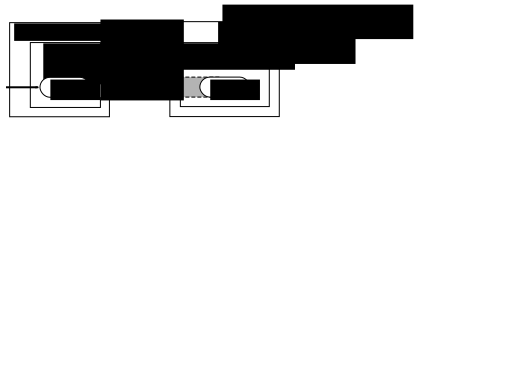
\includegraphics{./img/alsa-hw.svg.eps}
	\caption{{ALSA hw PCM plugin}}
	\label{fig:alsa-hw-plugin}
\end{figure}

When an ALSA application calls open API of PCM interface, this function read runtime configuration files and parse it. In ALSA default, /usr/share/alsa/alsa.conf is loaded at first. This file loads /usr/share/alsa/alsa.conf.d/*, /etc/asound.conf and ~/.asoundrc. As a result, for PCM runtime, several PCM nodes are available. For example, hw, plughw(plug plugin with hw slave), dmix, dsnoop and default, see Figure \ref{pcm-nodes-playback}.

\begin{figure}[htbp]
\small
\begin{verbatim}
$ aplay -L
default:CARD=PCH
    HDA Intel PCH, CX20590 Analog
    Default Audio Device
...
dmix:CARD=Intel,DEV=0
    HDA Intel, ALC889 Analog
    Direct sample mixing device
dsnoop:CARD=Intel,DEV=0
    HDA Intel, ALC889 Analog
    Direct sample snooping device
hw:CARD=Intel,DEV=0
    HDA Intel, ALC889 Analog
    Direct hardware device without any conversions
plughw:CARD=Intel,DEV=0
    HDA Intel, ALC889 Analog
    Hardware device with all software conversions
\end{verbatim}
\caption{ALSA PCM nodes for playback application}
\label{pcm-nodes-playback}
\end{figure}

\subsection{ALSA PCM plugins}
ALSA library has some PCM plugins for several purpose\footnote{src/pcm/ in alsa-lib} and dmix/dsnoop plugins are good exsamples for IPC usage in ALSA plugins. The dmix plugin multiplexes PCM frames from several applications and transfer the PCM frames to device. The dsnoop plugin delivers PCM frames from device to several applications. The dmix/dsnoop plugins use System V Shared Memory for IPC, System V Semaphore for mutual exclusive. ALSA PCM direct layer gives helper functions to these plugins.

\begin{figure}[htbp]
	\centering
	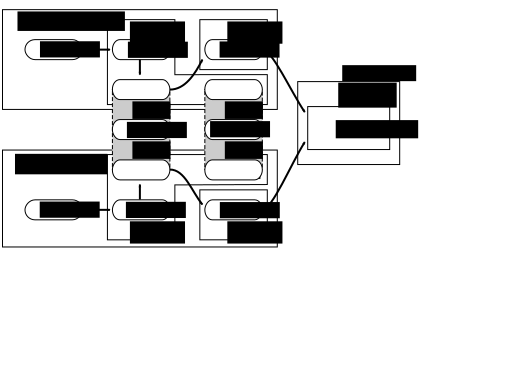
\includegraphics[scale=0.75]{./img/alsa-direct.svg.eps}
	\caption{ALSA dmix PCM plugin}
	\label{alsa_direct}
\end{figure}


When applications open dmix/dsnoop PCM node by calling snd\_pcm\_open(), the dmix/dsnoop plugins keep or connect System V Shared Memory and System V Semaphore. Then the shared memory is attached to the virtual memory space of each application process. This shared memory is used to share parameters and status of PCM substream for slave. The slave of dmix/dsnoop plugin is fixed to hw plugin. Additionally, the dmix plugin keeps one shared memory for multiplexing buffer, too.

When calling 'snd\_pcm\_writei()/snd\_pcm\_mmap\_commit()', the dmix plugin multiplexes PCM frames in application buffer and in shared memory, then write into slave buffer. The PCM frames are stored to shared memory and used by the other applications for next multiplexing. The shared memory is used as 'cache'. This allows any processes to multiplex PCM frames and write the frames to buffer for slave according to their timing. The buffer for slave is added by hw PCM plugin. The buffer is mmaped in process' virtual address space, therefore any processes can access the buffer (Figure \ref{fig:alsa-hw-plugin} to page \pageref{fig:alsa-hw-plugin}). The dmix plugin writes PCM frames, while this plugin doesn't move a buffer pointer by usual way so that any processes can write PCM frames into the same position.

The dsnoop PCM plugin is simpler than dmix PCM plugin because there's no need to multiplex PCM samples. Each application read PCM frames from shared memory.

There's two problems of ALSA PCM plugins for my purpose. The basic idea of ALSA PCM plugins is to add features to hw PCM node, therefore the framework for ALSA PCM plugins don't allow master without slave. The hw PCM node is for communication to drivers in kernel-land, therefore this is against my purpose in this section. Additionally, there's an issue that one of processes must handle packets. If an ALSA application perform this role, the application cannot stop as long as the other applications use PCM nodes for a firewire device. A daemon process, therefore, is required to handle packets for ALSA applications.


\subsection{ALSA External PCM plugins}
ALSA has another way to extend PCM nodes in runtime. It's External PCM Plugin\cite{alsa-lib}. There are two usages of this; Filter type and I/O type.

The Filter type plugin is similar to PCM plugins with master/slave, while I/O type plugin needs no slave. The I/O type, therefore, is good to communicate to a daemon process. A good example of I/O type plugin is pulse PCM External plugin\footnote{pulse/ in alsa-plugins} for PulseAudio.

PulseAudio\footnote{http://www.pulseaudio.org} is a project for sound server daemon. In modern desktop environment, PulseAudio adds ALSA runtime configuration\footnote{/usr/share/alsa/pulse-alsa.conf} to overwrite a default PCM node as pulse PCM node. As a result, most of applications in the desktop environment do IPC to PulseAudio via pulse External PCM plugin, then PulseAudio multiplexes/demultiplexes PCM samples for each ALSA applications. Finally, PulseAudio transfer PCM samples from/to each devices.

\begin{figure}[H]
	\centering
	\includegraphics[scale=0.5]{./img/alsa-pulse.dot.eps}
	\caption{ALSA pulse PCM plugin and PulseAudio}
	\label{alsa-pulse}
\end{figure}

PulseAudio implements several network protocols such like RTP-related protocols, and utilizes communication backends such like Rygel\footnote{Rygel is UPnP Device Architecture and Device Control Protocol application for Media Renderer/Server}. Furthermore, PulseAudio has its own network protocol to communicate to PulseAudio in the other hosts. This means that PulseAudio has a strong framework to use several types of devices.

There is another example. It's freebob External PCM Plugin for FreeBoB. The source of this plugin is in 'alsa-plugin' directory on the top of FFADO subversion trunk\footnote{http://subversion.ffado.org/browser/trunk}.

\begin{figure}[H]
	\centering
	\includegraphics[scale=0.5]{./img/alsa-freebob.dot.eps}
	\caption{{ALSA FreeBoB PCM plugin and Linux firewire subsystem}}
	\label{alsa_freebob}
\end{figure}

This plugin creates a thread when starting. This thread polls with libfreebob wait function, and transfers PCM samples/MIDI messages when waking up. This plugin also has a restriction that just one application can transfer streams, therefore either playback or capture is available. This plugin uses ALSA sequencer interface to gather/deliver MIDI messages between the other ALSA applications. This plugin seems to be under working and suspended but shows good perspective for ALSA applications to use FFADO.

The FreeBoB PCM plugin reinforces the requirement of daemon processes to packetize, because this plugin can't handle both of playback/capture PCM frames. In modern desktop environment, PulseAudio is a candidate for such daemon. If PulseAudio has firewire stack, ALSA applications can transfer data between firewire devices via default PCM node. For MIDI functionality, PulseAudio should use ALSA sequencer interface as FreeBoB plugin does.

But there's already a similar PCM External I/O plugin. It's jack PCM plugin for jackd. This plugin adds jack PCM node to ALSA runtime and make ALSA applications as a client for jackd. The jackd can use firewire devices with FFADO backend. This way requires users to write ALSA configuration but need no other works.

\begin{figure}[H]
	\centering
	\includegraphics[scale=0.5]{./img/alsa-jack.dot.eps}
	\caption{{ALSA JACK PCM plugin and JACK server daemon}}
	\label{alsa_jack}
\end{figure}

But there is a disadvantage of this way. When adding the configuration for jack plugin, the jack PCM node always exists in ALSA PCM runtime even if there is no process for jackd. This is not good at transparency for users.


\subsection{CUSE - Character device in user-space}
Linux Filesystem subsystem has CUSE as FUSE extension. CUSE allows to implement drivers for character devices in user-land.

\begin{figure}[H]
	\centering
	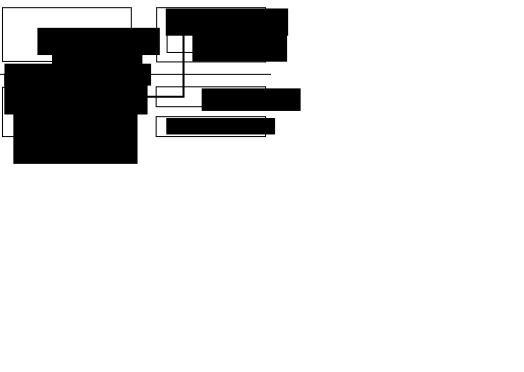
\includegraphics[scale=0.75]{./img/fuse.svg.eps}
	\caption{{FUSE/CUSE and user-land driver}}
	\label{fuse}
\end{figure}

Open Sound System Proxy Daemon (osspd) is a good example for CUSE application\footnote{http://sourceforge.net/projects/osspd/}. When Open Sound System applications access to Open Sound System character devices (/dev/dsp, /dev/mixer, /dev/adsp), osspd handles these file operations in user-space with CUSE help, then execute IPC between PulseAudio or ALSA.

\begin{figure}[H]
	\centering
	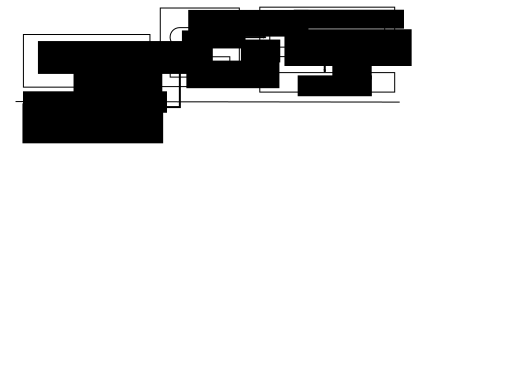
\includegraphics[scale=0.75]{./img/ossp-pulse.svg.eps}
	\caption{{Open Sound System Proxy Daemon}}
	\label{osspd_pulse}
\end{figure}


This daemon register Open Sound System character devices via FUSE library API. Then udev daemon adds the character devices to system according to rules which osspd adds. The daemon opens a pair of socket for IPC between daemon and slave, then creates a new process for the slave. The slave sleeps to wait IPC from the daemon, then do IPC between PulseAudio or ALSA.

For my purpose, this way is nice because there's no need to touch ALSA user-land implementation or ALSA runtime. But equivalent codes to whole ALSA Core should be implemented in the daemon to handle application's file operations. This needs much works. In this reason, the combination of 'light' ALSA driver in kernel-land and ALSA PCM component in user-land daemon is better.

\begin{figure}[H]
	\centering
	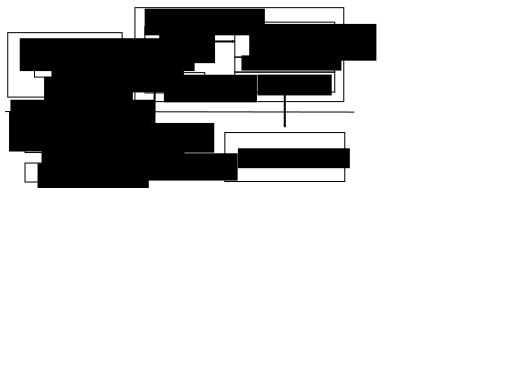
\includegraphics[scale=0.75]{./img/alsa-cuse-firewire.svg.eps}
	\caption{{User-land driver for ALSA and Firewire with CUSE}}
	\label{alsa_cuse_firewire}
\end{figure}

When device is connected, the driver registers ALSA character devices except for PCM. When system detects new ALSA devices for firewire sound devices, the system starts a daemon. The daemon calls FUSE library to add ALSA PCM character device with appropriate major/minor number. Then new PCM device is available in ALSA runtime. This idea can reduce the amount of codes in the daemon but still needs much works to implement ALSA PCM component in the daemon.

In this section, I investigate some software implementations in user-land to seek better ways for ALSA applications and firewire driver. As a result, I can conclude that the best way is to implement the drivers in PulseAudio, and realize the work is external to ALSA user-land. In the next section, I investigate ALSA kernel-land to seek another way.


\section{Investigation for kernel-land driver}

In this section, I investigate ALSA implementation in kernel-land.

Generally, after executing system-call, a process is running in kernel-mode and has a privilege to access hardware resources. If the data from hardware did not arrive yet, the process requests process-scheduler to generate context-switch. Then the another process gain CPU and continue to run. Before sleeping, the process registers an event for waking-up. Every time when requested to generate context-switch, process-scheduler checks the events and decide which process is awaken. This is a part of process-scheduling and dedicates to Time Sharing System (TSS).

When ALSA application executes system-call, the process in kernel-mode arrives at the codes in ALSA Core. ALSA Core includes some modules for each interface such as PCM. The code in these modules check events and continue the process if the event occurs, else it makes the process to sleep. When sound devices generate hardware interrupt, each ALSA driver handles the interrupt and generate a event. This is a simple explanation for ALSA implementation in kernel-land.

\subsection{ALSA Core and drivers}

ALSA Core consists of modules which perform important roles in sound subsystem. The source codes of ALSA Core locate under sound/core/. ALSA Core manages sound devices as 'card', and manages character devices corresponding to 'components' which belong to the card\cite{alsa-driver}. The component represents each functionality on sound devices such as PCM or MIDI, and the modules include helper functions for the components.

When a sound device is detected, a corresponding driver registers a instance of card to ALSA Core and adds instances of component to the card. Then ALSA Core requests Linux Driver Core to add character devices to system. When granting the request and handling it, Linux Driver Core registers the character devices and adds corresponding kobject, then notifies kevent. In usual desktop environment, "udevd" receives the kevent and adds special files to system for the character devices according to specific rules. Finally ALSA applications can communicate to components of drivers via the special files.

Major modules of ALSA Core are:

\begin{description}
\small
\item[snd] \mbox{} \\
Management of cards and devices, including methods for control interface, helper functions for control component and procfs nodes
\item[snd\_pcm] \mbox{} \\
Including methods for PCM interface and helper functions for PCM component
\item[snd\_rawmidi] \mbox{} \\
Including methods for MIDI interface and helper functions for MIDI component
\item[snd\_hwdep] \mbox{} \\
Including methods for hardware dependent interface and helper functions for hardware dependent component
\item[snd\_timer] \mbox{} \\
Including methods for timer interface and helper functions for timer component
\end{description}

These components include methods of common file operations such as ioctl or mmap, and defines a batch of ALSA-specific operations for drivers. Each driver registers functions as the methods at adding components. In this way, each driver becomes to handle requests from ALSA applications.

For communication to actual devices, drivers use each Linux subsystem because the devices are on buses such like PCI-Express bus or platform bus. The drivers should be registered to bus driver and handle callbacks from the bus driver. Additionally, data transmission is mostly based on DMA and related events are notified by hardware interrupt, therefore each driver should also uses Linux subsystem to handle DMA and hardware interrupt.

In next subsection, I describe interaction between PCM Interface/Component and application/driver.

\subsection{ALSA PCM Interface and PCM Component}
\label{sec:alsa-pcm}

ALSA PCM Interface and PCM Component are for transmission of PCM frames between applications and devices.

An instance of PCM Component includes two members for PCM streams. One is for an incoming stream and another is for an outgoing stream. The stream has several PCM substreams added by the drivers according to device's specification. For the substreams, ALSA Core adds PCM character devices. When applications open PCM character devices by PCM interface, corresponding PCM substream is opened and PCM runtime is attached to the substream.

The PCM runtime has several state, 'open', 'setup', 'prepared', 'running', 'xrun', 'draining', 'paused', 'suspended' and 'disconnected'\cite{alsa-lib}. Applications changes the state by PCM interface, then corresponding method of driver is called by PCM component. The runtime includes several information such like hardware description and hardware/software parameters. When the runtime is created, drivers set the hardware description in the runtime. Next, the application sets the hardware/software parameters by PCM interface.

When the parameters are decided, driver keeps PCM ring buffer. In most case, drivers support mmap file operation for PCM Component. Then PCM interface maps this buffer to process' virtual address area when applications or master plugins set mmap access flags to the hardware parameters\footnote{SND\_PCM\_ACCESS\_MMAP\_INTERLEAVED, SND\_PCM\_ACCESS\_MMAP\_NONINTERLEAVED and SND\_PCM\_ACCESS\_MMAP\_COMPLEX}.

The state of the ring buffer is in the other buffers; 'status' buffer and 'control' buffer. These buffers are kept by PCM Component in kernel-space when applications or master plugins open hw plugin. Then, in most case, 'hw\_ptr' and 'appl\_ptr' in these buffers are mapped to processes' virtual address area\footnote{When failed to mmap(2), an alternative way is applied. The hw plugin keeps a buffer for sync\_ptr structure. It execute ioctl(2) to update this pointer when any PCM frames are handled. This way includes overhead.}.

\begin{figure}
\small
\begin{verbatim}
struct snd_pcm_mmap_status {
        snd_pcm_state_t state;
        int pad1;
        snd_pcm_uframes_t hw_ptr;
        struct timespec tstamp;
        snd_pcm_state_t suspended_state;
        struct timespec audio_tstamp;
};
\end{verbatim}
\begin{verbatim}
struct snd_pcm_mmap_control {
        snd_pcm_uframes_t appl_ptr;
        snd_pcm_uframes_t avail_min;
};
\end{verbatim}
\caption{{Structures for ring buffer status and control}}
\label{pcm-mmap-status-control}
\end{figure}

The 'appl\_ptr' is updated only by applications. There's two cases. One of the cases is that some PCM frames are written or read by non-mmap functions\footnote{The functions are snd\_pcm\_writei() / snd\_pcm\_writen() / snd\_pcm\_readi() / snd\_pcm\_readn() but be sure to plugin-chain.}. In this case, PCM component moves the 'appl\_ptr' in kernel-space by the number of requested frames. Another case is that some PCM frames are committed by mmap functions\footnote{The function may be snd\_pcm\_mmap\_commit() but be sure to plugin-chain}. In this case, hw plugin changes the 'appl\_ptr' in user-space by the number of frames.

On the other hand, the 'hw\_ptr' is changed only by drivers when handling any hardware interrupts from devices. A page including 'hw\_ptr' is mapped in user-space as read-only, and no applications can change it. The 'hw\_ptr' is updated by the number of frames per 'period'. The 'period' is a part of ring buffer into which the ring buffer is split. When the devices confirm to finish transferring PCM frames by the number of period, they call snd\_pcm\_period\_elapsed(). Then the 'hw\_ptr' is moved to next beginning of period.

\begin{figure}[H]
	\centering
	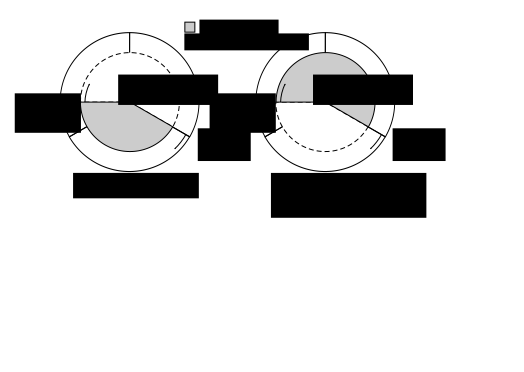
\includegraphics{./img/alsa-pcm-buffer.svg.eps}
	\caption{{PCM ring buffer}}
	\label{alsa-pcm-buffer}
\end{figure}

The two pointers, 'hw\_ptr' and 'appl\_ptr', are used to check 'avail' space for application. The 'avail' space is the number of frames currently available for applications. For playback application, the 'avail' space equals to a space in the ring buffer without PCM frames. For capture application, the 'avail' space equals to a space with PCM frames. When hw plugin writes or reads frames with non-blocking operation, functions instantly return if the 'avail' space has less frames than requested frames. When hw plugin writes or reads frames with blocking operation, the application is blocked until timeout or all of requested frames are transferred, or receiving signals. As a default, the timeout is 10 sec. The timeout means 'hw\_ptr' has never changed during the 10 sec, thus there may be some troubles about interrupt handler. But this behaviour is changed with 'NO\_PERIOD\_WAKEUP' hardware flag\footnote{SNDRV\_PCM\_HW\_PARAMS\_NO\_PERIOD\_WAKEUP} for PCM substream. If driver supports this functionality, the timeout is extended to the maximum number which Linux process-scheduler supports\footnote{MAX\_SCHEDULE\_TIMEOUT in include/linux/sched.h}. In this mode, hardware interrupts should be generated periodically and drivers are sure to handle them.

When applications executes poll(2) for descriptors gained by snd\_pcm\_poll\_descriptors() with hw plugin, by default the process is blocked till timeout or 'avail' space has a rest, or receiving signals. PCM Component has two modes for this behaviour; one is interrupt-base, as described, and another is a combination of both the interrupt-base and timer-base. When using the combination mode, snd\_pcm\_poll\_descriptors() returns two descriptors for both PCM character device and Timer character device. Both of them wake up per period but the source of timer is different. The way to change the mode is to set 'period\_event' software parameter for PCM runtime by snd\_pcm\_sw\_params\_set\_period\_event(). PulseAudio uses a combination of 'NO\_PERIOD\_WAKEUP' hardware parameter and 'period\_event' software parameter for its 'glitch free' operation\footnote{Features/GlitchFreeAudio http://fedoraproject.org/wiki/Features/GlitchFreeAudio}.

The rest of buffer against 'avail' is 'hw\_avail'. The 'hw\_avail' is available space for devices. For applications, the 'hw\_avail' is the space for rewinding. The applications can reverse 'appl\_ptr' by the number of frames in 'hw\_avail'. But developers should be sure that 'hw\_ptr' can be changed by drivers in any time.

The actual value for these two pointers doesn't round up in the number of frames in buffer. It's incremented until 'boundary' within UINT\_MAX, then round up. The way to calculate the 'boundary' is:

\begin{equation}
boundary = UINT\_MAX - UINT\_MAX / frames\_per\_buffer 
\end{equation}

\begin{figure}[H]
	\centering
	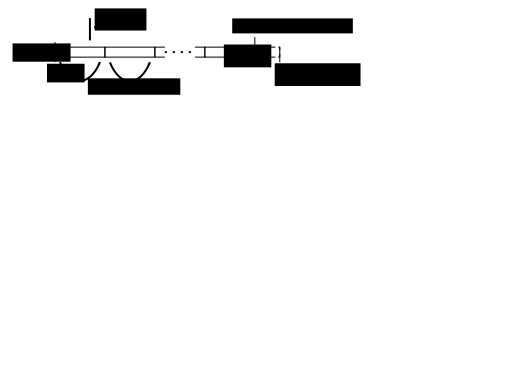
\includegraphics{./img/alsa-buffer-boundary.svg.eps}
	\caption{{PCM buffer boundary}}
	\label{alsa--buffer-boundary}
\end{figure}


\subsection{Linux firewire subsystem}

ALSA firewire stack uses Linux firewire subsystem to communicate to firewire devices. Before investigating ALSA firewire stack, I describe Linux firewire subsystem.

Linux firewire subsystem, so-called Juju\footnote{I don't know the reason.}, is IEEE 1394 and OHCI 1394 application and support these functionalities:

\begin{itemize}
\small
\item IEEE 1394 Serial bus management
\item IEEE 1394 Transaction layer
\item Driver for OHCI 1394 compliant controller device
\item Driver for fw character device corresponding to units
\end{itemize}

This subsystem locates under drivers/firewire/ and consists of several files. They include snoop mode driver for a certain 1394 controller, and protocol drivers for RFC 2734\footnote{https://tools.ietf.org/html/rfc2734 IPv4 over IEEE 1394}, RFC 2855\footnote{https://tools.ietf.org/html/rfc2855 DHCP for IEEE 1394}, RFC 3146\footnote{https://tools.ietf.org/html/rfc3146 Transmission of IPv6 Packets over IEEE 1394 Networks } and SBP-2. But here I describe core functionality and OHCI 1394 related stuff only:

\begin{description}
\small
\item[drivers/firewire/core-cdev.c] \mbox{} \\
Methods for file operations of fw character devices
\item[drivers/firewire/core-device.c] \mbox{} \\
Helper functions for management of units
\item[drivers/firewire/core-topoligy.c] \mbox{} \\
Management of bus topology by reaction to events on the bus
\item[drivers/firewire/core-iso.c] \mbox{} \\
Helper functions to handle isochronous context
\item[drivers/firewire/core-transaction.c] \mbox{} \\
Helper functions to handle asynchronous context
\item[drivers/firewire/core-card.c] \mbox{} \\
Abstract layer for host controller devices
\item[drivers/firewire/ohci.c] \mbox{} \\
Driver for OHCI 1394 compliant host controller
\end{description}

\begin{figure}[htbp]
	\centering
	\includegraphics[scale=0.5]{./img/fw-stack-high.dot.eps}
	\caption{{Linux firewire subsystem (a higher part)}}
	\label{fw-stack-high}
\end{figure}

This subsystem performs Cycle Master and Bus Manager in IEEE 1394. This subsystem adds fw character devices for applications. The fw character devices are corresponding to each unit on IEEE 1394 bus. The applications in user-land can communicate to the units by executing file operations to the fw character devices, mainly ioctl(2). As ALSA does, this subsystem also gives a library (libraw1394) for API as an abstract layer for the specific file operations. Additionally, this subsystem also gives API for kernel-land.

The functionalities for Asynchronous Communication and Isochronous Communication are based on OHCI 1394. Thus, they are represented as context (section \ref{ohci-1394} to page \pageref{ohci-1394}).

Linux firewire stack has an abstract layer for the controller device. Currently two drivers are under this abstract layer. The dummy driver is mainly used to shutdown actual cards, therefore OHCI 1394 driver is usually used to communicate actual devices. This driver receives/transmits data of packet from/to controller by DMA according to descriptors, and handle hardware interrupts which the controller generates. The driver controls the controller via registers.

\begin{figure}[htbp]
	\centering
	\includegraphics[scale=0.5]{./img/fw-stack-low.dot.eps}
	\caption{{Linux firewire subsystem (a lower part) and host controller}}
	\label{fw-stack-low}
\end{figure}

\subsection{ALSA firewire stack}

ALSA firewire stack is designed for each driver to communicate to firewire devices via Linux firewire subsystem. ALSA firewire stack locates under sound/firewire/. This stack includes helper functions for IEC 61883-1/6:

\begin{description}
\small
\item[sound/firewire/iso-resources.c] \mbox{} \\
   Helper functions to manage isochronous resources
\item[sound/firewire/cmp.c] \mbox{} \\
   For Connection Management Procedure (CMP) in IEC 61883-1
\item[sound/firewire/lib.c] \mbox{} \\
   Helper functions for asynchronous transaction
\item[sound/firewire/fcp.c] \mbox{} \\
   For Function Control Protocol (FCP) in IEC 61883-1
\item[sound/firewire/packets-buffer.c] \mbox{} \\
   Helper functions to manage buffer for continuous packets
\item[sound/firewire/amdtp.c] \mbox{} \\
   For AMDTP packet streaming in IEC 61883-6
\end{description}

All of them are used to built for 'snd-firewire-lib' module. While firewire sound drivers use the helper functions to communicate to sound devices, the drivers also use ALSA Core to communicate to ALSA applications.

\begin{figure}[htbp]
	\centering
	\includegraphics[scale=0.5]{./img/alsa-stack.dot.eps}
	\caption{{ALSA Core and firewire stack}}
	\label{alsa_stack}
\end{figure}

\subsubsection{Isochronous Resources functionality}

This module gives a structure for isochronous resources such as channels and bandwidth. Drivers initialize an instance of the structure by fw\_iso\_resources\_init() with firewire unit. After initializing, the drivers can allocate/free isochronous resources by fw\_iso\_resources\_allocate()/fw\_iso\_resources\_free(). When bus reset occurs, fw\_iso\_resources\_update() should be called. To release the instance, fw\_iso\_resources\_destroy() is used.

\subsubsection{CMP functionality}

This module gives a structure for CMP operation. This functionality uses the isochronous resources functionality internally. Drivers initialize an instance of the structure by cmp\_connection\_init(). To keep bandwidth/channels and establish a connection, cmp\_connection\_establish() is used with maximum number of bytes for payload of a packet, and cmp\_connection\_break() is used to break the connection. To release the instance, cmp\_connection\_destroy() is used after breaking the connection. When bus reset occurs, cmp\_connection\_update() is used to update the connection.

As of 2013, this functionality supports operations for iMPR/iPCR for input connections.

\subsubsection{FCP and transaction functionality}

FCP functionality gives a function, fcp\_avc\_transaction() for FCP and AV/C commands. The drivers can transmit FCP request and wait for FCP response for 125 millisecond. All of FCP requests should be retried when bus reset occurs. For this purpose, fcp\_bus\_reset() is used.

FCP functionality internally uses snd\_fw\_transaction(). This is a wrapper function of fw\_run\_transaction() and supports retrying and generation constraint.


\subsubsection{Continuous packets buffer functionality}

This module gives a structure for continuous packet buffer. Drivers initialize an instance of the structure by iso\_packets\_buffer\_init() with the number of packets and the number of bytes in an packet. After initialized, the instance has pages to queue packets. To release the instance, iso\_packets\_buffer\_destroy() is used.

\subsubsection{AMDTP functionality}
\label{sec:packetization-out}

This module gives a structure and some operations to handle an instance of the structure for AMDTP outgoing stream. This functionality uses the continuous packets buffer functionality internally. Drivers initialize an instance of the structure by amdtp\_out\_stream\_init(). After initializing, amstp\_out\_stream\_set\_parameters() is used to set streaming parameters such as sampling rate, the number of MBLA data channel and MIDI Conformant data channel. After setting these parameters, amdtp\_out\_stream\_get\_max\_payload() returns the maximum number of bytes in payload for a packet with current parameters.

Drivers can start the stream by amdtp\_out\_stream\_start(). Then amdtp\_out\_stream\_stop() is used to stop the stream. To release the stream, amdtp\_out\_destroy\_stream() is used. When bus reset occurs, amdtp\_out\_stream\_update() is used for new node ID.

For PCM component, snd-firewire-lib gives helper functions. Before starting streaming, amdtp\_out\_stream\_set\_pcm\_format() is used to set PCM format. To initialize PCM-related members of a stream, amdtp\_out\_stream\_pcm\_prepare() is used. When starting/stopping to transfer PCM frames, amdtp\_out\_stream\_pcm\_trigger() is used. To get the numbers of frames in PCM ring buffer, amdtp\_out\_stream\_pcm\_pointer() is used. When killing PCM substreams, amdtp\_out\_stream\_pcm\_abort() is used. To check whether PCM substream is running or not over an AMDTP stream, amdtp\_out\_stream\_pcm\_running() is used.

Let's see the detail to generate AMDTP outgoing packets in Figure \ref{fig:packetization-out}. At first, the amdtp\_out\_stream\_start() function queues a series of packet with a 'skip' flag, then firewire-ohci adds the packets into descriptor list. To the end of the series, the function sets 'interrupt' flag. When the 'interrupt' packet is queued, firewire-ohci sets special flag to a descriptor corresponding to the packet. After queueing, the amdtp\_out\_stream\_start() function starts an isochronous context with a callback function. Then firewire-ohci starts to transfer descriptors to OHCI 1394 controller via DMA, and OHCI 1394 controller transmits packets corresponding to the descriptors. When OHCI 1394 controller finish transmitting the 'interrupt' packet, it generates hardware interrupt. The firewire-ohci handles the interrupt and schedules tasklet. When the tasklet is executed in software interrupt context, the callback function is executed. Then snd-firewire-lib generates new series of packets with PCM samples, and queueing them. At the end of packets in the series, the functionality sets the 'interrupt' flag again. When OHCI 1394 controller transmits this packet, it generates hardware interrupt and snd-firewire-lib generates new series of packets and queues them.

\begin{figure}[H]
	\centering
	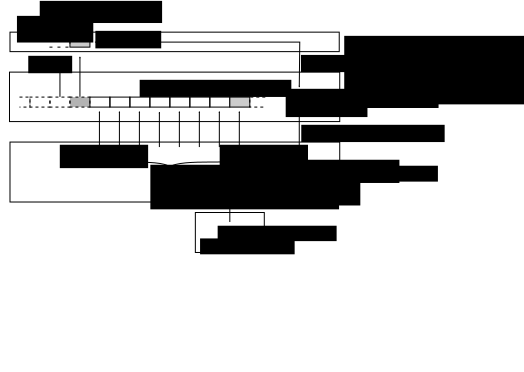
\includegraphics{./img/packetization-out.svg.eps}
	\caption{{Generating packets for outgoing stream}}
	\label{fig:packetization-out}
\end{figure}

As of 2013, AMDTP functionality uses 48 queues \footnote{QUEUE\_LENGTH in sound/firewire/amdtp.c} and 16 packets for interrupt interval \footnote{INTERRUPT\_INTERVAL in sound/firewire/amdtp.c}. The hardware interrupts nominally occur every 2 millisecond and it takes 6 millisecond to transmit a first packet with PCM frames since starting isochronous context. Actual interval depends on bandwidth usage (see Figure \ref{fig:cycle-start} to page \pageref{fig:cycle-start})and tasklet scheduling.

There is a case that snd-firewire-lib fails to continue streaming. It's to fail queueing packets. To check whether a stream is running or not, amdtp\_out\_stream\_running() is used, and amdtp\_out\_streaming\_error() is used to detect error. Once streaming becomes error state, the stream should be stopped by amdtp\_out\_stream\_stop(), then start by amdtp\_out\_stream\_start() again.

As of 2013, this functionality doesn't allow drivers to perform as a timing slave. Although a timing slave is required to handle the sequence of value in SYT field from incoming packets to outgoing packets (Section \ref{sec:duplex-streams} to page \pageref{sec:duplex-streams}), the functionality doesn't support incoming packets. The functionality, therefore, includes the generators of the sequence of value in SYT field and the number of data blocks in each packets because these sequences are relevant to each other.

\section{Enhancement of ALSA firewire stack}

As of 2013, this stack is only for AMDTP outgoing stream (received stream in device side) in both blocking/non-blocking mode. In detail,
\begin{itemize}
\item CMP functionality handles iMPR/iPCR only
\item AMDTP functionality handles isochronous outgoing context only
\item AMDTP packets can transfer PCM frames only
\item The value of SYT field in packets from device is not available for outgoing packet
\end{itemize}

To support more devices, this stack requires these functionalities:
\begin{itemize}
\item Handling oMPR/oPCR
\item Handling isochronous incoming context
\item Handling several data in an AMDTP packet, like MIDI
\item Handling duplex streams with timestamp synchronization
\end{itemize}

Additionally, each driver requires these functionalities:
\begin{itemize}
\item Retrieving device capabilities and parsing them to make PCM runtime rules
\item Maintaining duplex streams
\item PCM component for both of playback and capture
\item MIDI component for both of playback and capture
\item Handling model specific operations and quirks
\end{itemize}

Furthermore, each driver should prevent from disturbing user-land drivers. Dice driver already gives these functionalities via hwdep interface:
\begin{itemize}
\item Giving firewire node information corresponding to ALSA card
\item Notifying to start/stop streaming
\item Locking/Unlocking streaming
\end{itemize}

Comparing to an idea to implement drivers in user-land, an idea to implement it in kernel-land has less issues of communication to ALSA application because this idea can use ALSA Core. This idea gives good transparency to ALSA applications. Moreover, there's already ALSA firewire stack for firewire drivers. The stack has a lack of some requirements, while an enhancement of the stack is less work than implementing it in user-land.

I started the works for this idea in the beginning of 2013, and the works are merged to ALSA upstream May 2014. It takes one and a half years. June 2014, at Linux 3.16 merge window, ALSA maintainer pushed the work into Linux upstream. The patchset for the work consists of many patches. The first 18 patches are for snd-firewire-lib, AMDTP, CMP and FCP. The next 14 patches are for fireworks driver. The next 16 patches are for bebob driver. The rest of patches are for correction.

\subsection{Enhancement for AMDTP}

The snd-firewire-lib newly supports these functionalities for AMDTP:

\begin{itemize}
	\item Handling incoming AMDTP stream
	\item PCM capturing support
	\item MIDI capturing/playbacking support
	\item AMDTP data channel mapping
	\item duplex streams with timestamp synchronization
\end{itemize}

This work renames prefix of 'amdtp\_out\_stream' to 'amdtp\_stream' for all of functions and members for AMDTP stream structure, to use the same structure and functions for both directions.

This work newly adds a support for AMDTP incoming stream, and adds an argument for amdtp\_stream\_init(), to indicate the direction of AMDTP stream. After initialized, the instance of stream can be operated by the same way for both direction.

Let's see the detail to handle AMDTP incoming stream in Figure \ref{fig:packetization-in}. The mechanism is almost the same as generating outgoing packets, while there are two big differences.

One is dequeueing packets instead of generating packets. When OHCI 1394 controller fills an 'interrupt' descriptor with an incoming packet, it generates a hardware interrupt. The firewire-ohci handles this hardware interrupt and schedules tasklet. When the tasklet is executed in software interrupt context, a callback function in snd-firewire-lib is executed. Then AMDTP functionality perform dequeueing and queueing packets.

In current implementation, the length of queue and the interval of interrupt is the same for incoming/outgoing AMDTP stream. As a result, it nominally takes 2 millisecond to handle a first incoming packet since the packet reached.

Another is a functionality to detect discontinuity of the sequence of incoming AMDTP packets. Each AMDTP packet has DBC field for this purpose. In a case of the detection, the stream is stopped and corresponding PCM substream is aborted. In this case, the stream should be stopped and started again.

\begin{figure}[H]
	\centering
	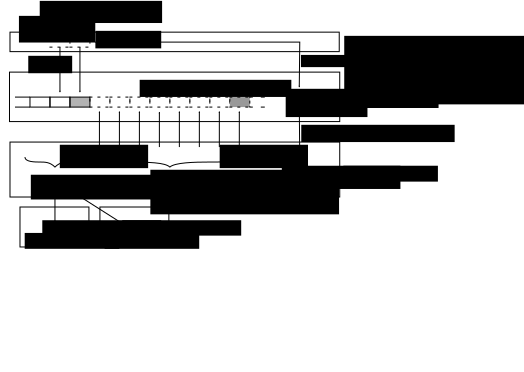
\includegraphics{./img/packetization-in.svg.eps}
	\caption{{Handling packets for incoming stream}}
	\label{fig:packetization-in}
\end{figure}

This work newly adds amdtp\_stream\_wait\_callback() to wait for a first packet until given timeout. This is for detection of the case that drivers set wrong parameters for packets, i.e. a wrong tag for IEEE 1394 isochronous packet. In this case, OHCI 1394 driver doesn't execute callback function in isochronous context. Then no packets are handled, and PCM component don't waken a process of PCM substream because 'avail' space has never been updated (section \ref{sec:alsa-pcm} to page \pageref{sec:alsa-pcm}). This function is expected to be used just after staring a stream, to prevent from this case. Drivers should handle error state when receive false.

This work adds some flags for AMDTP stream structure, to handle device's quirks of stream. Between initializing and starting a stream, these flags can be set to an instance of the stream. Fireworks and BeBoB drivers use these flag.

By default, any AMDTP streams are not associated. For duplex streams with timestamp synchronization (section \ref{sec:duplex-streams} to page \pageref{sec:duplex-streams}), amdtp\_stream\_set\_sync() is added to associate two streams as a timing master and a timing slave with given synchronization mode, and this function should be called before starting streams. Currently CIP\_SYNC\_TO\_DEVICE is effective for this parameter and for AMDTP stream in blocking mode. The case to use this option is that a timing master is incoming stream and a timing slave is outgoing stream. In this case, the value of SYT field in incoming packets are passed to outgoing packets. The packets in both direction are handled in interrupt context for an incoming isochronous context. Hence, a callback in isochronous context for outgoing stream is ignored. In the other cases, there's no requirement to pass the value of SYT field between two streams.

\begin{figure}[H]
	\centering
	
\includegraphics{./img/packetization-duplex.svg.eps}
	\caption{{Handling associated duplex streams}}
	\label{fig:packetization-duplex}
\end{figure}


In IEC 61883-6\cite{iec61883-6-1, iec61883-6-2} and MMA/AMEI RP-027\cite{amei-rp27}, one MIDI Conformant data channel supports 8 MIDI substreams. This work newly adds a support of this multiplexed MIDI substream in AMDTP stream. During streaming, each drivers can trigger MIDI messages with amdtp\_stream\_midi\_trigger(). Some models ignore MIDI messages in more than 8 data blocks in an packet. This may be due to a gap of data rate between MIDI bus and IEEE 1394 bus. To handle this quirk, struct amdtp\_stream.rx\_blocks\_for\_midi is used.

For PCM component, this work newly adds amdtp\_stream\_add\_hw\_constraints() to add PCM constraint according to parameters of AMDTP stream. This function should be called after all of needed flags are set to an instance of AMDTP stream structure.

This work allows drivers to call amdtp\_stream\_set\_pcm\_format() during a stream is running. This is for the case that PCM substream is going to join in AMDTP stream which MIDI substream already starts.

\subsection{Enhancement for CMP}

This work adds an argument to cmp\_connection\_init(), to indicate direction. After initializing, the instance of CMP is handled as what it was.

Each driver can read iPCR/oPCR by transaction in any time. To confirm no drivers handle the device, cmp\_connection\_check\_used() is used. This is a consideration about user-land driver. I also proposed the same idea for FFADO\footnote{[FFADO-devel] Adjustment between FFADO/ALSA for Firewire drivers  http://sourceforge.net/p/ffado/mailman/message/31856195/}.

I note that the value of payload field in oPCR is not used to keep bandwidth because some device chip reports a wrong value. Instead of this, snd-firewire-lib uses the value of data\_block\_quadlets member in struct amdtp\_stream.

\subsection{Enhancement for FCP}

This work enables firewire-lib to handle deferred transaction. According to AV/C General specification\cite{avc-general-4-2}, receivers of AV/C command should respond to transmitter within 100 millisecond, while the receivers send an intermediate response within 100 millisecond and send a final response later. This is deferred transaction. The interval between the intermediate and the final response is undefined. But to promise to return to caller, 125 millisecond interval is used.

Additionally, this work adds three AV/C commands, which seems to be used in some drivers. They are INPUT/OUTPUT SIGNAL FORMAT command and PLUG INFO command in AV/C General\cite{avc-general-4-2}.

\section{Driver implementation}

The enhancement of ALSA firewire stack allows to implement new drivers and to update existed drivers. In this section, I describe about specifications of these drivers.

\subsection{Common specifications}

The drivers for Fireworks/BeBoB/OXFW/Dice utilize ALSA firewire stack, therefore they have common specifications for each component.

\subsubsection{PCM component}

An instance of PCM component in each driver has SND\_PCM\_INFO\_BATCH flag because AMDTP functionality uses several packet buffers to transfer PCM frames (section \ref{sec:alsa-pcm} to page \pageref{sec:alsa-pcm}).

PCM component also has SND\_PCM\_INFO\_BLOCK\_TRANSFER flag because PCM frames are transferred at each interrupt by the number of data blocks in some packets \footnote{INTERRUPT\_INTERVAL in /sound/firewire/amdtp.c}.

PCM frames are copied to each data blocks in its order and the position of PCM frames in a data block is linear, thus SNDRV\_PCM\_INFO\_INTERLEAVED should be used.

If devices supports both streams, in most case, incoming/outgoing AMDTP streams should be the same sampling rate, thus SNDRV\_PCM\_INFO\_JOINT\_DUPLEX should be used. Each drivers should restrict sampling rate for both playback/capture as the same. If current source of clock is not internal or recovered clock (section \ref{sec:clock-recovery} to page \pageref{sec:clock-recovery}), the sampling rate should not be changed.

Currently, SNDRV\_PCM\_HW\_PARAMS\_NO\_PERIOD\_WAKEUP is not used because these drivers have a possibility to stop streaming suddenly due to failure of packet queueing or detection of packet discontinuity. In this case, process with the flag is kept blocking.

The number of channels in each PCM substream depends on the number of MBLA data channels in data block of AMDTP packet. The number is different depending on models even if the models use the same device chipset (Section \ref{sec:formation-data-block} to page \pageref{sec:formation-data-block}).

Fireworks/BeBoB/OXFW/Dice ignores labels of AM824 data, thus each drivers handle IEC 60958 Conformant data channel as MBLA data channel for simple implementation\footnote{[alsa-devel] [PATCH] firewire-lib: Use IEC 61883-6 compliant labels for Raw Audio data http://mailman.alsa-project.org/pipermail/alsa-devel/2014-June/077326.html}.

\subsubsection{MIDI component}

MIDI functionality is supported. Most devices have a pair of input/output port but a few devices have several ports. Currently AMDTP functionality supports one MIDI Conformant data channel \footnote{AMDTP\_MAX\_CHANNELS\_FOR\_MIDI in sound/firewire/amdtp.h}, thus the maximum number of MIDI ports is restricted by 8.

\subsubsection{Hwdep component}
Hwdep functionality is used to the same purpose as Dice driver uses. ALSA applications can execute I/Os to this interface. The API is in include/uapi/sound/firewire.h. The requests are:

\begin{description}
\small
\item [SNDRV\_FIREWIRE\_IOCTL\_GET\_INFO] \mbox{} \\
This request returns data of struct snd\_firewire\_get\_info. This information tells the type of driver, firewire card index, GUID for the device and name of fw character device like "fw1,0".
\item [SNDRV\_FIREWIRE\_IOCTL\_LOCK] \mbox{} \\
This request locks the driver's functionality of streaming for user-land driver.
\item [SNDRV\_FIREWIRE\_IOCTL\_UNLOCK] \mbox{} \\
This request unlocks the driver's functionality of streaming for user-land driver.
\end{description}

Furthermore, ALSA hwdep applications can receive notifications by reading hwdep interface. The notification is a form of union snd\_firewire\_event. Each kind of this union has "type" member in its first field and tells the type of event to ALSA hwdep applications. The event to starting/stopping streaming by drivers are commonly implemented and the other events depend on each driver.

\subsubsection{Control component}
Control functionality is used just to get card information, because the drivers basically add no control elements. ALSA control applications, therefore, cannot control device's DSP behaviour (section \ref{sec:internal-mixing} to page \pageref{sec:internal-mixing}). This functionality can be implemented in user-land. For this purpose, currently, ffado-dbus-server/ffado-mixer are one of recommendations.

\subsubsection{Proc information}

To help debug, the drivers add proc nodes under the card's "firewire" subdirectory. When reporting bugs, users should also reports output from these nodes. These nodes should not be used fot the other purposes.


\subsection{Fireworks driver}

Fireworks driver locates in sound/firewire/fireworks/ and consists of 9 files. When initializing, the driver registers a handler into a certain address on host controller to receive responses of Fireworks transaction. Currently the maximum length of Fireworks transaction is 304 bytes (for isochronous channel mapping), therefore 512 bytes are allocated for the handler including enough space. Fireworks has a command to change the address, although the driver uses the default address for each model because the address space on host controller is an exclusive resource and it's preferable to allocate as small as possible. The structure of Fireworks transaction is in include/uapi/sound/firewire.h.

\begin{figure}[H]
\small
\begin{verbatim}
#define SNDRV_FIREWIRE_EVENT_EFW_RESPONSE       0x4e617475
struct snd_firewire_event_efw_response {
        unsigned int type;
        __be32 response[0];     /* some responses */
};

#define SND_EFW_TRANSACTION_USER_SEQNUM_MAX     ((__u32)((__u16)~0) - 1)
/* each field should be in big endian */
struct snd_efw_transaction {
        __be32 length;
        __be32 version;
        __be32 seqnum;
        __be32 category;
        __be32 command;
        __be32 status;
        __be32 params[0];
};
\end{verbatim}
\caption{API for Fireworks transaction}
\label{uapi-fireworks-transaction}
\end{figure}

ALSA hwdep applications can transmit a request by writing to hwdep interface. Each instance of fireworks driver has a queue to store the responses and ALSA hwdep applications can read them via hwdep interface. There is a rule for the request that ALSA hwdep applications must use the correct value for 'seqnum' member between 0 to SND\_EFW\_TRANSACTION\_USER\_SEQNUM\_MAX because the value out of the range is used by the driver itself. I note that the driver implements needed commands to maintain streams or help debug. You can see most kinds of fireworks transaction in FFADO\footnote{http://subversion.ffado.org/browser/trunk/libffado/src/fireworks/efc}.

Fireworks has two modes to transmit AMDTP packets; Window mode and IEC 61883 mode. In Windows mode, the value of dbc in first CIP header is zero and whole the second CIP header is used to indicate timestamp. Another is IEC 61883 mode but this is not fully compliant to IEC 61883-1/6. Additionally, Fireworks has the other quirks. To support such quirks, the driver apply several flags to amdtp structure, while CMP is used by an usual way.

Fireworks has a quirk at bus reset, to restart dbc from zero. To handle this quirk, the driver doesn't check packet continuity when dbc is zero.

\subsection{BeBoB driver}

BeBoB driver locates under sound/firewire/bebob/ and consists of 12 files. To handle vendor specific operation, the driver has several files for each vendor. Especially, M-Audio largely customized their models and two of them\footnote{Firewire 1814 and ProjectMix I/O} have many specific operations. The two models also has write-only controls, therefore the driver adds control elements for the two, as only an exception.

BeBoB has a quirk at bus reset. It transmits packets with disorder just after bus reset. To recover from this discontinuity, the driver uses completion to serialize PCM component .prepare() call and firewire subsystem .update() call.

\subsection{OXFW driver}

OXFW driver may be newly added as a successor of firewire-speakers driver. The driver may be move to sound/firewire/oxfw/ and split to 9 files. Originally, firewire-speakers driver supports PCM playback and two models, while OXFW driver may support more models and PCM/MIDI playback and capture.

The firewire-speakers driver supports ALSA control elements for two models, thus OXFW driver may still support this interface for them. But for the other models, OXFW driver may not give this interface. Ideally, this functionality should be move to user-land.

\subsection{Dice driver}

Dice driver may be moved to sound/firewire/dice/ and split to 9 files. Originally, the driver supports PCM playback only but may be extended to PCM/MIDI playback and capture.

Dice has its own mechanism to notify status change, therefore the driver gives a way to read the notification via hwdep interface. It's implemented as a type of event. ALSA hwdep applications read the event and parse it to know current status.

\begin{figure}[H]
\small
\begin{verbatim}
#define SNDRV_FIREWIRE_EVENT_DICE_NOTIFICATION   0xd1ce004e
struct snd_firewire_event_dice_notification {
        unsigned int type;
        unsigned int notification; /* DICE-specific bits */
};
\end{verbatim}
\caption{API for Dice notification}
\label{uapi-dice-notification}
\end{figure}

The driver allocate a handler to a specific address on host controller when probing each device. The length of Dice notification is just 4 bytes, therefore, it's reasonable to allocate an address for each device.

Dice has a quirk at bus reset not to react any transactions for reconnection. In this reason, the driver stops any streams at bus reset.

\section{Rest of issue}

Currently I focus on enabling ALSA to handle the devices. There are still some issues which don't cause big problems.

\subsection{OXFW and Dice enhancement}

I already posted patches for these drivers \footnote{[alsa-devel] [RFC][PATCH 00/15 v4] OXFW driver, a successor to firewire-speakers \\ http://mailman.alsa-project.org/pipermail/alsa-devel/2014-May/076581.html} \footnote{[alsa-devel] [RFC][PATCH 00/13 v1] Enhancement for Dice driver \\ http://mailman.alsa-project.org/pipermail/alsa-devel/2014-May/076730.html}. The previous revision of OXFW driver \footnote{It's a part of [alsa-devel] [RFC v3] [PATCH 00/52] Enhancement for support of firewire devices http://mailman.alsa-project.org/pipermail/alsa-devel/2014-January/071820.html} has a regression for a device. The device has several entries for stream formation at a certain sampling rate, then parser of driver brought this regression. Dice enhancement adds supports for duplex streams with timestamp synchronization and playback/capture of PCM/MIDI.

I don't have the device confirmed with regression and any Dice based devices. I really need testers.

\subsection{A lack of arrangement for severe latency}
Currently, the minimum number of frames per period is not less than the amount equals to 5 millisecond. PCM component of each driver has a flag, SNDRV\_PCM\_INFO\_BATCH, thus the minimum number of periods in buffer is 2 because its hw\_ptr is changed at each interrupt. As a result, the minimum latency is over 10 millisecond. For severe latency, the size of period should be as smaller as possible.

Ideally, the number of PCM frames in a period should be the number of data blocks in packets handled by one interrupt so as a PCM period is corresponds to an interrupt (section \ref{sec:alsa-pcm} to page \pageref{sec:alsa-pcm}). In both of blocking and non-blocking modes, the number of data blocks in each packet is different, while current implementation apply fixed number of packets as an interval of interrupt. The fixed interval of interrupt brings periods without any interrupt, see Figure \ref{fig:interrupt-period}. In this figure, sampling transfer frequency is 44.1kHz, thus the interval of SYT is 8 data blocks. The number of packets in an interrupt is fixed to 4, the number of PCM frames in an period is 16. In blocking mode, PCM period is elapsed two times in 3rd interrupt. In non-blocking mode, PCM period is elapsed two times in 5th interrupt.

\begin{figure}[H]
	\centering
	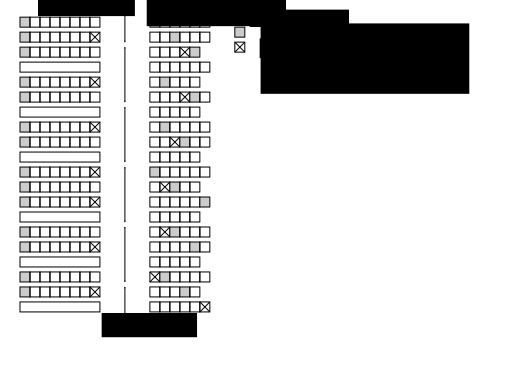
\includegraphics{./img/interrupt-period.svg.eps}
	\caption{{Sequences of packets, interrupts and PCM periods}}
	\label{fig:interrupt-period}
\end{figure}

Current implementation uses 5 milliseconds to ensure that at least one interrupt occurs between PCM periods. To apply severe latency, the interrupt interval should be changed dynamically according to sampling transmission frequency and the number of frames in a period. But this needs correct calculation and estimation for the number of packets till next PCM period.


\subsection{A lack of delay for timestamp processing}

When incoming/outgoing streams are associated and a device is a clock master, a driver uses the value of SYT field in incoming packet for the field in outgoing packet. If the master and slave handle the same value of SYT field in the same timing, the outgoing packet should include additional delay by the number of data blocks in packets in a queue. 

Current implementation simply copies the value. I have no issues about this with Fireworks/BeBoB/OXFW. To consider maintenance effort, it may be better to keep it what it is.

\subsection{A lack of PCM configuration for virtual surround nodes}

ALSA library has configuration files for each PCM component of sound card\footnote{Usually under /usr/share/alsa/cards/.}. These configuration files have settings for virtual PCM nodes. Some of these nodes are for surround channels such as "front", "side", "surround40" and so on. PulseAudio uses these nodes to decide available mapping for channels.

Such settings use "route" PCM plugin to resolve a mismatch between the number of actual channels and channels requested by ALSA PCM application. The plugin is designed to have the actual number of channels for its parameters in each configuration file.

But most of firewire devices newly supported have a different number of channels depending on models, sampling frequency and a certain modes even if they utilizes the same device chipset (Section \ref{sec:formation-data-block} to page \pageref{sec:formation-data-block}). In this reason, "route" PCM plugin is not available for the settings of these devices, while it's better to add no configuration files to ALSA library for each model because this idea requires ALSA developers to maintain 100 or more files\footnote{For example, "FWSpeakers.conf" and "FireWave.conf" were added to ALSA library 1.0.25, while they are based on OXFW970/971.}.

Instead of "route" PCM plugin, "plug" PCM plugin is available for this purpose. The plugin needs no parameters for actual channels. The plugin can resolve the mismatch of channels, as long as ALSA PCM applications open PCM nodes without "SND\_PCM\_NO\_AUTO\_CHANNELS" flag.

Unfortunately, PulseAudio uses the flag. PulseAudio fails all of trials to detect channel mapping, therefore it cannot handle the devices\footnote{[pulseaudio-discuss] 'Failed to find a working profile' for firewire sound devices http://lists.freedesktop.org/archives/pulseaudio-discuss/2014-January/019685.html}.

Furthermore, most of these firewire devices have settings for DSP (Section \ref{sec:internal-mixing}). ALSA PCM functionality can cause silence when the settings is wrong. For example, there is a device which receives AMDTP packets with 10 MBLA data channels and an ALSA application uses it as a device with stereo channels. Even if ALSA PCM functionality correctly push PCM samples into the first two data channels and fill zero PCM samples in the rest of data channels, the device can generate no sound or sound in unexpected audio ports according to the settings.

As a result, the variety of data channel make it difficult to unified configuration files, and DSP settings weaken a practical meaning of the configuration. In these reasons, current ALSA library has no configuration files for the firewire devices newly supported.

\subsection{A lack of throttles for MIDI messages in outgoing stream}
In MIDI specification, its physical layer can transfer 31,250 bit per second. This equals to 3,906 Byte per second. But in IEC 61883-6\cite{iec61883-6-1, iec61883-6-2} and MMA/AMEI RP-027\cite{amei-rp27}, AMDTP stream can transfer MIDI messages by one eighth of sampling transmit frequency (STF). This is really much than MIDI specification, therefore devices must buffer the gap between these data rate.

\begin{table}[H]
	\centering
	\caption{{Data rate for MIDI message over IEEE 1394 bus}}
	\label{tbl:midi-rate}
	\begin{tabular}{cc} \toprule
		STF	& Byte per second \\ \midrule
		32,000	& 4,000.0	\\
		44,100	& 5,512.5	\\
		48,000	& 6,000.0	\\
		88,200	& 11,025.0	\\
		96,000	& 12,000.0	\\
		176,400	& 22,050.0	\\
		192,000	& 24,000.0	\\ \bottomrule
	\end{tabular}
\end{table}

A few devices have buffer-over-flow when receiving much MIDI messages. For example, M-Audio Firewire 1814 transfer discontinuous packets when receiving much MIDI messages. There are some devices which ignores MIDI messages in more than first 8 data blocks in a packet and this seems to be a solution for this issue in vendor side.

In this reason, ALSA Firewire stack should have a throttle for MIDI messages in outgoing stream.

\subsection{A lack of control elements for ALSA control interface}

Firewire sound devices needs software implementation to control their DSP behaviour (section \ref{sec:internal-mixing} to page \pageref{sec:internal-mixing}) or device specific features.

The most devices have some ports for audio input and output. Additionally, they can receive some MBLA data channels (section \ref{sec:internal-mixing} to page \pageref{sec:internal-mixing}). Each input from audio ports and MBLA data channels can be multiplexed to each port to audio output. Furthermore, the ratio to multiplex each input to each output is changeable. As a result, this multiplexing functionality has routing settings by the number of available inputs multiplied by the number of available outputs. In FFADO, this feature is called as 'matrix mixer'.

Moreover, some devices have its specific features; phantom powering or hardware metering. The way to control these feature depends on models.

ALSA firewire drivers basically have no ALSA control interface elements because this functionality can be implemented in user-land as FFADO does. Moreover, a few devices have write-only controls, hence there is a need of permanent storage. Current ALSA control interface has no mechanism for the storage.

Currently, ffado-dbus-server/ffado-mixer is one of recommendations for this purpose but they are isolated from ALSA applications. There is an issue for transparency to ALSA applications again.

Like ALSA PCM interface, ALSA control interface has External Control plugins. It may be possible to give ways to control DSP for ALSA applications with the plugin.

A control element for the matrix mixer requires 4 parameters; sink ID, source ID, ratio. For this purpose, 'byte' type of ALSA control interface element is better with a certain structure. The plugin should inform the number of sinks/sources and the range of ratio to ALSA control applications.

If it is OK to use no control elements via control interface, it is better to implement this functionality in alsa-tools package, like envy24 or HDSP. 

Anyway, further investigation and discussion are needed for this issue.


\subsection{A lack of packet sorting}
Some Fireworks based devices sometimes transfer packets with disorder, see Figure \ref{fireworks-disorder}. Such sequence of packet is detected as discontinuity and firewire-lib stop streaming.

I've already posted my solution for this issue\footnote{[alsa-devel] [PATCH 09/39] firewire-lib: Add sort function for transmitted packet http://mailman.alsa-project.org/pipermail/alsa-devel/2014-March/073875.html} but this is rejected by a maintainer due to three points:
\begin{itemize}
\item AMDTP is nearly real-time protocol, thus it's not acceptable to have a delay of processing packets.
\item The solution apply general way to sort, while this quirk is currently confirmed only on Fireworks, thus no need to apply general way.
\item A certain pattern is confirmed to the discontinue sequence of packets. It's possible to add a few codes just for this quirk.
\end{itemize}

\begin{figure}[htbp]
\small
\begin{verbatim}
Index   Payload CIP header 1    CIP header2
032     002     3F110028        90FFFFFF
033     210     3F110030        900410E8
034     210     3F110038        900424E8
035     210     3F110040        900438E8
036     002     3F110040        90FFFFFF
037     210     3F110050 <-     900464E8
038     210     3F110048 <-     900450E8
039     210     3F110058        900478E8
040     002     3F110058        90FFFFFF
041     210     3F110068 <-     9004A4E8
042     210     3F110060 <-     900490E8
043     210     3F110070        9004B8E8
044     002     3F110070        90FFFFFF
045     210     3F110080 <-     9004E4E7
046     210     3F110078 <-     9004D0E8
\end{verbatim}
\caption{A sample of packets with disorder transmitted by Fireworks}
\label{fireworks-disorder}
\end{figure}

I confirm the disorder occurs less times than correct order. Further investigation is needed for better solution.

\subsection{A few devices freeze when frequent establishing/breaking connections}
'PreSonus FP10' can freeze when frequent establishing/breaking connections. This brings a disadvantage to PulseAudio. When PulseAudio detects the card, it starts/stops 4 streams at least. Currently PulseAudio cannot detect devices with non-surround channels. But when making PulseAudio detects the device with dbus rule and PulseAudio profiles, it may take the device freezing.

\subsection{Various results at bus reset}
Various results are confirmed with Fireworks/BeBoB at bus reset. They are depending on cases:
\begin{description}
\item{Case 1. Software bus reset} \mbox{} \\
When generating bus reset with ffado-test or jujuutils\footnote{https://code.google.com/p/jujuutils/}, streaming stopped suddenly. When generating bus reset, the drivers update connections according to IEC 61883-1. But after a few hundred millisecond, the device break connections by itself. I don't know the reason exactly but I guess the synchronizing mechanism I described has some relations.
\item{Case 2. Connecting devices or removing devices on the bus} \mbox{} \\
This case depends on which devices are connected or removed. If they are Fireworks/BeBoB based devices, streaming sometimes continues and sometimes stops. If they are not Fireworks/BeBoB based device, streaming continues. I don't know the reason exactly but I guess the synchronizing mechanism I describe have some relations. 
\end{description}

\subsection{A lack of synchronizing several devices on the same bus}
As long as reading manual of PreSonus/Focusrite/PrismSound for BeBoB based devices, there is a way to synchronize devices on the same bus. This mechanism is based on clock recovery, therefore it's driven by handling the value of SYT field in CIP packets:
\begin{itemize}
\item Driver selects a device as 'Sample clock source' then the other devices are 'Sample clock destination'.
\item Driver handles packets from the source device.
\item Driver reads SYT and calculate presentation timestamp for each devices, then transfer packets to the destination devices.
\item Driver sets recovered clock as sampling clock source for the destinations, in advance.
\end{itemize}

IEC 61883-6:2005\cite{iec61883-6-2}describes actual examples in Annex D.1.3 Embedded sample-clock jitter.

Currently ALSA Firewire stack doesn't support this mechanism. The reason is a bad balance between actual cost to implement its requirements and actual advantage to implement them. The requirements are:
\begin{itemize}
\item Requirement to manage states of several devices simultaneously
\item Requirement to handle several streams from/to all devices simultaneously
\end{itemize}

Instead of this type of synchronization, ALSA Firewire stack handle packets from a device and read SYT, then transfer packets with the value to the device. I believe this is enough for general use cases.

\newpage

\begin{thebibliography}{99}

\addcontentsline{toc}{section}{References}

\bibitem{ieee1394-1}
IEEE 1394-1995 IEEE Standard for a High Performance Serial Bus
\bibitem{ieee1394-1-a}
IEEE 1394a-2000 IEEE Standard for a High Performance Serial Bus - Amendment 1
\bibitem{ieee1394-1-b}
IEEE 1394b-2002 IEEE Standard for a High Performance Serial Bus - Amendment 2
\bibitem{ieee1394-1-c}
IEEE 1394c-2006 IEEE Standard for a High Performance Serial Bus - Amendment 3
\bibitem{ieee1394-2}
IEEE 1394-2008 IEEE Standard for a High Performance Serial Bus

\bibitem{ieee1212-1}
IEEE 1212-1991: IEEE Standard Control and Status Register (CSR) Architecture for Microcomputer Buses
\bibitem{iso13213}
ISO/IEC 13213:1994 Information technology -- Microprocessor systems -- Control and Status Registers (CSR) Architecture for microcomputer buses
\bibitem{ieee1212-2}
IEEE 1212-2001: IEEE Standard Control and Status Register (CSR) Architecture for Microcomputer Buses

\bibitem{amdtp-1}
TA Document 1997001 Audio and Music Data Transmission Protocol Version 1.0
\bibitem{amdtp-1-1}
TA Document 1999014 Enhancement to Audio and Music Transmission Protocol Version 1.0 (July 10, 2000, 1394TA)
\bibitem{amdtp-2}
TA Document 2001003 Audio and Music Data Transmission Protocol 2.0
\bibitem{amdtp-2-1}
TA Document 2001024 Audio and Music Data Transmission Protocol 2.1 (May 24, 2002, 1394TA)

\bibitem{amei-rp27}
MMA/AMEI RP-027 MIDI Media Adaptation Layer for IEEE-1394 Version 1.0 (Nov 30 2000)

\bibitem{iec61883-1-1}
IEC 61883-1:1998 Consumer audio/video equipment - Digital interface - Part 1: General, Edition 1.0
\bibitem{iec61883-1-2}
IEC 61883-1:2003 Consumer audio/video equipment - Digital interface - Part 1: General, Edition 2.0
\bibitem{iec61883-1-3}
IEC 61883-1:2008 Consumer audio/video equipment - Digital interface - Part 1: General, Edition 3.0

\bibitem{iec61883-6-1}
IEC 61883-6:2002 Consumer audio/video equipment - Digital interface - Part 6: Audio and Music Data Transmission Protocol, Edition 1.0
\bibitem{iec61883-6-2}
IEC 61883-6:2005 Consumer audio/video equipment - Digital interface - Part 6: Audio and Music Data Transmission Protocol, Edition 2.0

\bibitem{ohci1394-1}
1394 Open Host Controller Interface Specification Release 1.0 (Oct 20 1997)
\bibitem{ohci1394-1-1}
1394 Open Host Controller Interface Specification Release 1.1 (Jan 06 2000)

\bibitem{avc-general-4-2}
TA Document 2004006, AV/C Digital Interface Command Set General Specification Version 4.2 (September 1, 2004, 1394TA)
\bibitem{avc-audio-1}
TA Document 1999008, AV/C Audio Subunit 1.0 (August 21, 2000, 1394TA)
\bibitem{avc-connection-1}
TA Document 2002010, AV/C Connection and Compatibility Management Specification 1.1
\bibitem{avc-music-1}
TA Document 2001007, AV/C Music Subunit 1.0 (April 8, 2001, 1394TA)
\bibitem{avc-descriptor-1}
TA Document 1999025, AV/C Descriptor Mechanism Specification Version 1.0 (July 23, 2001, 1394TA)
\bibitem{avc-info-block-1}
TA Document 1999045, AV/C Information Block Types Specification Version 1.0 (July 23, 2001, 1394TA)
\bibitem{avc-general-enhancement}
TA Document 2000004, Enhancements to the AV/C General Specification 3.0 Version 1.1 (Oct 24, 2000, 1394TA)
\bibitem{avc-stream-format-1}
AV/C Stream Format Information Specification V1.0
\bibitem{avc-stream-format-1-1}
TA Document 2004008, AV/C Stream Format Information Specification 1.1 (working draft) (April 15, 2005, 1394TA)
\bibitem{avc-rate-control}
TA Document 1999015, AV/C Command Set for Rate Control of Isochronous Data Flow 1.0

\bibitem{icelynx}
Using TSB43Cx43A: S/PDIF Over 1394 (Dec 2003, Texas Instruments Incorrporated)
\bibitem{bebob-1}
Additional AVC commands - AV/C Unit and Subunit - SDD Products Draft 1.7-00 (Nov 17 2003, BridgeCo)
\bibitem{bebob-2}
AV/C Connection Management - Implementation Recommendation - SDD Products Draft 4.0-01 (Jul 16 2004, BridgeCo AG)

\bibitem{alsa-lib}
ALSA Library API \\
http://www.alsa-project.org/main/index.php/ALSA\_Library\_API
\bibitem{alsa-driver}
Writing an ALSA Driver (2005, Takashi Iwai) \\
http://www.alsa-project.org/main/index.php/ALSA\_Driver\_Documentation

\end{thebibliography}

\newpage

\appendix

\addcontentsline{toc}{section}{Appendices}
\addtocontents{toc}{\protect\setcounter{tocdepth}{-1}}

\section{Functions of Linux firewire subsystem}

ALSA firewire stack utilize functions exported by Linux firewire stack. In this appendix, I describe the functions.

\subsection{Serial Bus Management}

\begin{verbatim}
void fw_iso_resource_manage(struct fw_card *card, int generation,
                            u64 channels_mask, int *channel,
                            int *bandwidth, bool allocate);
\end{verbatim}

This function allocates or deallocates a channel and/or bandwidth for resources of isochronous communication by transactions to CSR\_CHANNELS\_AVAILABLE and CSR\_BANDWIDTH\_AVAILABLE in Isochronous Resource Manager.

\begin{verbatim}
void fw_schedule_bus_reset(struct fw_card *card, bool delayed,
                           bool short_reset);
\end{verbatim}

This function schedules bus reset on OHCI 1394 controller.

\subsection{Firewire subsystem transaction services}

\begin{verbatim}
typedef void (*fw_address_callback_t)(struct fw_card *card,
                                      struct fw_request *request,
                                      int tcode, int destination, int source,
                                      int generation,
                                      unsigned long long offset,
                                      void *data, size_t length,
                                      void *callback_data);
struct fw_address_handler {
        u64 offset;
        u64 length;
        fw_address_callback_t address_callback;
        void *callback_data;
        struct list_head link;
};
struct fw_address_region {
        u64 start;
        u64 end;
};
int fw_core_add_address_handler(struct fw_address_handler *handler,
                                const struct fw_address_region *region);
void fw_core_remove_address_handler(struct fw_address_handler *handler);
\end{verbatim}

The 'fw\_core\_add\_address\_handler' allocates an address region to the handler. If the address space is not already allocated or the address space is for FCP, the allocation is success. The callback in the handler is called when receiving transactions to the address space.

\begin{verbatim}
void fw_send_response(struct fw_card *card,
                      struct fw_request *request, int rcode);
int fw_cancel_transaction(struct fw_card *card,
                          struct fw_transaction *transaction);
\end{verbatim}

The 'fw\_send\_response()' and 'fw\_cancel\_transaction()' are used in the callback of the handler to send response or cancel the transaction.

\begin{verbatim}
int fw_run_transaction(struct fw_card *card, int tcode, int destination_id,
                       int generation, int speed, unsigned long long offset,
                       void *payload, size_t length);
\end{verbatim}

The 'fw\_run\_transaction()' is used to send asynchronous transaction to the node.

\subsection{OHCI 1394 isochronous contexts}

\begin{verbatim}
struct fw_iso_buffer {
        enum dma_data_direction direction;
        struct page **pages;
        int page_count;
        int page_count_mapped;
};
int fw_iso_buffer_init(struct fw_iso_buffer *buffer, struct fw_card *card,
                       int page_count, enum dma_data_direction direction);
void fw_iso_buffer_destroy(struct fw_iso_buffer *buffer, struct fw_card *card);
\end{verbatim}

This structure describes DMA mapped pages for OHCI 1394 isochronous context. The payload of each IEEE 1394 isochronous packet is stored in this buffer. 

\begin{verbatim}
struct fw_iso_context *fw_iso_context_create(struct fw_card *card,
                        int type, int channel, int speed, size_t header_size,
                        fw_iso_callback_t callback, void *callback_data);
\end{verbatim}

This function keeps isochronous context on OHCI 1394 host controller, then allocate DMA buffers for OHCI 1394 packet descriptor and IEEE 1394 isochronous packet header. The caller must allocate channel and bandwidth in advance.

\begin{verbatim}
struct fw_iso_packet {
        u16 payload_length;
        u32 interrupt:1;
        u32 skip:1;
        u32 tag:2;
        u32 sy:4;
        u32 header_length:8;
        u32 header[0];
};
\end{verbatim}

This structure basically represents IEEE 1394 Isochronous Packet. An 'interrupt' member is to generate from hardware interrupt of OHCI 1394. If the value of 'interrupt' member is 1 in every 16 packets, it means that the hardware interrupt is generated every 16 packets handled by OHCI 1394 controller.

\begin{verbatim}
int fw_iso_context_queue(struct fw_iso_context *ctx,
                         struct fw_iso_packet *packet,
                         struct fw_iso_buffer *buffer,
                         unsigned long payload);
\end{verbatim}

This function queueing given a packet to isochronous context with the buffer. The members of 'struct fw\_iso\_packet' are copied to DMA buffer for OHCI 1394 descriptor.

\begin{verbatim}
void fw_iso_context_queue_flush(struct fw_iso_context *ctx);
\end{verbatim}

This function wakes up isochronous context with queued packets.

\begin{verbatim}
int fw_iso_context_flush_completions(struct fw_iso_context *ctx);
\end{verbatim}

This function generates software interrupt (tasklet) for isochronous context.

\begin{verbatim}
int fw_iso_context_start(struct fw_iso_context *ctx,
                         int cycle, int sync, int tags);
\end{verbatim}

This function takes isochronous context to start.

\begin{verbatim}
int fw_iso_context_stop(struct fw_iso_context *ctx);
\end{verbatim}

This function takes isochronous context to stop and disable software interrupt (tasklet).

\begin{verbatim}
void fw_iso_context_destroy(struct fw_iso_context *ctx);
\end{verbatim}

This function takes isochronous context to stop and disable software interrupt, then release isochronous context and deallocate buffer.

\newpage

\section{Functions of ALSA firewire stack}

In this appendix, I describe functions of ALSA firewire stack in detail.

\subsection{Continuous packets helper functions}

These functions are in sound/firewire/iso-packets.\{c,h\}.

\begin{verbatim}
struct iso_packets_buffer {
        struct fw_iso_buffer iso_buffer;
        struct {
                void *buffer;
                unsigned int offset;
        } *packets;
};
int iso_packets_buffer_init(struct iso_packets_buffer *b, struct fw_unit *unit,
                            unsigned int count, unsigned int packet_size,
                            enum dma_data_direction direction);
void iso_packets_buffer_destroy(struct iso_packets_buffer *b,
                                struct fw_unit *unit);
\end{verbatim}

This structure includes 'struct fw\_iso\_buffer' and non-tag structure. The non-tag structure consists of pointer and offset to access the content of memory pages in packet unit. The 'iso\_packets\_buffer\_init()' function calculates the number of memory page frames with 'packet\_size' argument, 'count' argument, L1\_CACHE\_ALIGN() and PAGE\_SIZE, then keeps the pages for DMA with 'fw\_iso\_buffer\_init()'. The 'iso\_packets\_buffer\_destroy()' releases the structure.

\subsection{Isochronous Resource Management helper functions}

These functions are in sound/firewire/iso-resources.\{c,h\}.

\begin{verbatim}
struct fw_iso_resources {
        u64 channels_mask;
        struct fw_unit *unit;
        struct mutex mutex;
        unsigned int channel;
        unsigned int bandwidth;
        unsigned int bandwidth_overhead;
        int generation;
        bool allocated;
};
int fw_iso_resources_init(struct fw_iso_resources *r,
                          struct fw_unit *unit);
void fw_iso_resources_destroy(struct fw_iso_resources *r);
int fw_iso_resources_allocate(struct fw_iso_resources *r,
                              unsigned int max_payload_bytes, int speed);
int fw_iso_resources_update(struct fw_iso_resources *r);
void fw_iso_resources_free(struct fw_iso_resources *r);
\end{verbatim}

The structure 'fw\_iso\_resources' represents an manager for isochronous resource such like channel and bandwidth. The 'fw\_iso\_resources\_init()' initializes it and 'fw\_iso\_resources\_destroy()' release it.
The 'fw\_iso\_resources\_allocate()' keeps isochronous resources with given 'max\_payload\_bytes' and 'speed'. The 'fw\_iso\_resources\_update()' reallocate isochronous resources to handle bus reset. The 'fw\_iso\_resources\_free()' releases isochronous resources. Most operations utilizes 'fw\_iso\_resource\_manage()' in Linux firewire subsystem.

\subsection{CMP helper functions}

These functions are written in sound/firewire/cmp.\{c,h\}.

\begin{verbatim}
enum cmp_direction {
        CMP_INPUT = 0,
        CMP_OUTPUT,
};
struct cmp_connection {
        int speed;
        bool connected;
        struct mutex mutex;
        struct fw_iso_resources resources;
        __be32 last_pcr_value;
        unsigned int pcr_index;
        unsigned int max_speed;
        enum cmp_direction direction;
};
int cmp_connection_init(struct cmp_connection *connection,
                        struct fw_unit *unit,
                        enum cmp_direction direction,
                        unsigned int pcr_index);
int cmp_connection_check_used(struct cmp_connection *connection, bool *used);
void cmp_connection_destroy(struct cmp_connection *connection);
int cmp_connection_establish(struct cmp_connection *connection,
                             unsigned int max_payload);
int cmp_connection_update(struct cmp_connection *connection);
void cmp_connection_break(struct cmp_connection *connection);
\end{verbatim}

The 'struct cmp\_connection' includes parameters related to CMP such like PCR index. The 'cmp\_connection\_init()' check Output/Input MPR by a READ transaction according to given 'direction' and 'pcr\_index', then initialize 'resources' member. The 'cmp\_connection\_destroy()' release these structures. The 'cmp\_connection\_establish()' keeps isochronous resources and establishes a connection by a LOCK transaction. The 'cmp\_connection\_update()' updates a connection by a LOCK transaction to handle bus reset. The 'cmp\_connection\_break()' breaks an established connection by a LOCK transaction. The connection should be broken before destroyed.

The 'cmp\_connection\_check\_used()' is a bit special. This is added for relationships to drivers in user-space. When the drivers handle devices, the caller of this function can check the driver's connection.

\subsection{AMDTP stream helper functions}

These functions are in sound/firewire/amdtp.\{c,h\}.

\begin{verbatim}
enum amdtp_stream_direction {
        AMDTP_OUT_STREAM = 0,
        AMDTP_IN_STREAM
};
enum cip_flags {
        CIP_NONBLOCKING         = 0x00,
        CIP_BLOCKING            = 0x01,
        CIP_SYNC_TO_DEVICE      = 0x02,
        CIP_EMPTY_WITH_TAG0     = 0x04,
        CIP_DBC_IS_END_EVENT    = 0x08,
        CIP_WRONG_DBS           = 0x10,
        CIP_SKIP_DBC_ZERO_CHECK = 0x20,
        CIP_SKIP_INIT_DBC_CHECK = 0x40,
        CIP_EMPTY_HAS_WRONG_DBC = 0x80,
};
struct amdtp_stream {
        struct fw_unit *unit;
        enum cip_flags flags;
        enum amdtp_stream_direction direction;
        struct fw_iso_context *context;
        struct mutex mutex;

        struct iso_packets_buffer buffer;
        int packet_index;

        enum cip_sfc sfc;
        unsigned int syt_interval;

        unsigned int source_node_id_field;
        unsigned int data_block_quadlets;
        unsigned int data_block_counter;
        unsigned int pcm_channels;
        unsigned int midi_ports;
        u8 pcm_positions[AMDTP_MAX_CHANNELS_FOR_PCM];
        u8 midi_position;

        unsigned int tx_dbc_interval;

        unsigned int transfer_delay;
        unsigned int data_block_state;
        unsigned int last_syt_offset;
        unsigned int syt_offset_state;

        struct amdtp_stream *sync_slave;

        bool callbacked;
        wait_queue_head_t callback_wait;

        struct snd_pcm_substream *pcm;
        void (*transfer_samples)(struct amdtp_stream *s,
                                 struct snd_pcm_substream *pcm,
                                 __be32 *buffer, unsigned int frames);
        unsigned int pcm_buffer_pointer;
        unsigned int pcm_period_pointer;
        bool pointer_flush;
        struct tasklet_struct period_tasklet;

        struct snd_rawmidi_substream *midi[AMDTP_MAX_CHANNELS_FOR_MIDI * 8];
        unsigned int rx_blocks_for_midi;
};
\end{verbatim}

This structure represents an AMDTP stream. Currently this structure is for AM824 data. An AMDTP stream can transfer one PCM substream and 8 MIDI substreams. The 'buffer' member is for continuous packet buffer, and the 'index' member is for handling the continuous packets. The 'sfc' and 'syt\_interval' are dominant parameters. These parameters are decided by stream's nominal sampling rate:

\begin{verbatim}
enum cip_sfc {
        CIP_SFC_32000  = 0,
        CIP_SFC_44100  = 1,
        CIP_SFC_48000  = 2,
        CIP_SFC_88200  = 3,
        CIP_SFC_96000  = 4,
        CIP_SFC_176400 = 5,
        CIP_SFC_192000 = 6,
        CIP_SFC_COUNT
};
extern const unsigned int amdtp_syt_intervals[CIP_SFC_COUNT] = {
        [CIP_SFC_32000]  =  8,
        [CIP_SFC_44100]  =  8,
        [CIP_SFC_48000]  =  8,
        [CIP_SFC_88200]  = 16,
        [CIP_SFC_96000]  = 16,
        [CIP_SFC_176400] = 32,
        [CIP_SFC_192000] = 32,
};
\end{verbatim}


The 'source\_node\_id\_field', 'data\_block\_quadlets', 'data\_block\_counter' are for CIP header. The 'tx\_dbc\_interval' is for a device-specific quirk which has fixed interval for the value of data block counter, not compliant to IEC 61883-1.

The 'transfer\_delay', 'data\_block\_state', 'last\_syt\_offset', 'syt\_offset\_state' are used to generate the value of SYT field in non-blocking mode without timestamp synchronization. The 'sync\_slave' is used for blocking mode with duplex streams with timestamp synchronization to handle timestamps in incoming packets to outgoing packets.

The 'callbacked' and 'callback\_wait' are used to wait till a first packet is available.

The 'pcm' and 'transfer\_samples' members are used to multiplex/demultiplex PCM samples into an AMDTP packet. The 'pcm\_buffer\_pointer', 'pcm\_period\_pointer', 'pointer\_flush', 'period\_tasklet' are used to call 'snd\_pcm\_period\_elapsed()' in period boundary.

The 'midi' member is used to multiplex/demultiplex MIDI message into an AMDTP packet. The 'rx\_blocks\_for\_midi' is for a model-specific quirk to ignore MIDI messages in data blocks more than a certain numbers in a packet.

\begin{verbatim}
bool cip_sfc_is_base_44100(enum cip_sfc sfc);
\end{verbatim}

The 'cip\_sfc\_is\_base\_44100()' returns given 'sfc' is 44100, 88200, 176400 or not.

\begin{verbatim}
int amdtp_stream_init(struct amdtp_stream *s, struct fw_unit *unit,
                      enum amdtp_stream_direction dir,
                      enum cip_flags flags);
\end{verbatim}

The 'amdtp\_stream\_init()' initializes members in the structure. This function gets reference counter from given 'struct fw\_unit'. The 'dir' and 'flags' are important for an AMDTP stream.

\begin{verbatim}
void amdtp_stream_destroy(struct amdtp_stream *s);
\end{verbatim}

The 'amdtp\_stream\_destroy()' clear some members in the structure. This function put reference counter to given 'struct fw\_unit'. The caller is sure to stop the stream in advance.

\begin{verbatim}
void amdtp_stream_set_parameters(struct amdtp_stream *s,
                                 unsigned int rate,
                                 unsigned int pcm_channels,
                                 unsigned int midi_ports);
\end{verbatim}

The 'amdtp\_stream\_set\_parameters()' sets parameters to given stream structure. As a result, the stream structure has values in 'sfc', 'syt\_interval', 'pcm\_channels', 'midi\_ports', 'data\_block\_quadlets', 'transfer\_delay' fields. This function also initializes 'pcm\_positions' and 'midi\_positions' according to IEC 61883-6:2005.

\begin{verbatim}
unsigned int amdtp_stream_get_max_payload(struct amdtp_stream *s);
\end{verbatim}

The 'amdtp\_stream\_get\_max\_payload()' returns the number of bytes as maximum size of payload of CIP for an AMDTP packet. The caller must call 'amdtp\_stream\_set\_parameters()' in advance.

\begin{verbatim}
void amdtp_stream_set_sync(enum cip_flags sync_mode,
                           struct amdtp_stream *master,
                           struct amdtp_stream *slave);
\end{verbatim}

As a default, the synchronization mode is simplex stream without timestamp synchronization. The 'amdtp\_stream\_set\_sync()' set synchronization mode between master and slave streams for duplex streams with timestamp synchronization.

\begin{verbatim}
int amdtp_stream_start(struct amdtp_stream *s, int channel, int speed);
bool amdtp_stream_wait_callback(struct amdtp_stream *s, unsigned int timeout);
\end{verbatim}

The 'amdtp\_stream\_start()' starts an amdtp stream over given channel and speed. Then Linux Firewire subsystem start isochronous context and to handle related interrupts. The 'amdtp\_stream\_wait\_callback()' is to wait till a first packet can be available or timeout with given value.

\begin{verbatim}
bool amdtp_stream_running(struct amdtp_stream *s);
bool amdtp_streaming_error(struct amdtp_stream *s);
\end{verbatim}

The 'amdtp\_stream\_running()' is to check whether the stream is running or not. The 'amdtp\_streaming\_error()' is to check whether the stream is stopped with errors. The reasons of error is described later in this chapter.

\begin{verbatim}
void amdtp_stream_update(struct amdtp_stream *s);
\end{verbatim}

The 'amdtp\_stream\_update' is used to update the 'source\_node\_id\_field' member, basically to handle bus reset. Internally, amdtp\_stream\_start() also calls this function.

\begin{verbatim}
void amdtp_stream_stop(struct amdtp_stream *s);
\end{verbatim}

The 'amdtp\_stream\_stop' stops and destroys isochronous context, to stop an AMDTP stream. Then this function releases the buffer for continuous packets.

\subsection{PCM substream helper functions for AMDTP stream}

\begin{verbatim}
#define AMDTP_IN_PCM_FORMAT_BITS        SNDRV_PCM_FMTBIT_S32
#define AMDTP_OUT_PCM_FORMAT_BITS       (SNDRV_PCM_FMTBIT_S16 | \
                                         SNDRV_PCM_FMTBIT_S32)
\end{verbatim}

These macro is for 'struct snd\_pcm\_hardware.formats'. This represents current firewire-lib capability.

\begin{verbatim}
#define AMDTP_MAX_CHANNELS_FOR_PCM      64
\end{verbatim}

This macro represents the maximum number of PCM channels which current firewire-lib can handle.

\begin{verbatim}
int amdtp_stream_add_pcm_hw_constraints(struct amdtp_stream *s,
                                        struct snd_pcm_runtime *runtime);
\end{verbatim}

This function adds constraints to given PCM substream runtime according to given stream.

\begin{verbatim}
void amdtp_stream_set_pcm_format(struct amdtp_stream *s,
                                 snd_pcm_format_t format);
\end{verbatim}

The 'amdtp\_stream\_set\_pcm\_format()' sets 'transfer\_samples' member into stream according to given format. This is expected to be called in 'struct snd\_pcm\_ops.hw\_params()'.

\begin{verbatim}
void amdtp_stream_pcm_prepare(struct amdtp_stream *s);
\end{verbatim}

The 'amdtp\_stream\_pcm\_prepare()' initializes members related to handling 'snd\_pcm\_period\_elapsed()'. This is expected to be called in 'struct snd\_pcm\_ops.prepare()'.

\begin{verbatim}
unsigned long amdtp_stream_pcm_pointer(struct amdtp_stream *s);
\end{verbatim}

The 'amdtp\_stream\_pcm\_pointer()' returns the number of frames in an PCM ring buffer.

\begin{verbatim}
void amdtp_stream_pcm_trigger(struct amdtp_stream *s,
                              struct snd_pcm_substream *pcm);
\end{verbatim}

The 'amdtp\_stream\_pcm\_trigger()' sets 'pcm' member to given AMDTP stream. This is expected to be called in 'struct snd\_pcm\_ops.trigger'.

\begin{verbatim}
void amdtp_stream_pcm_abort(struct amdtp_stream *s);
\end{verbatim}

The 'amdtp\_stream\_pcm\_abort()' stops PCM substream with XRUN state. This is expected to be used before stopping AMDTP stream.

\begin{verbatim}
bool amdtp_stream_pcm_running(struct amdtp_stream *s);
\end{verbatim}

The 'amdtp\_stream\_pcm\_running()' is to check whether PCM substreams is running on the AMDTP stream or not.


\subsection{MIDI substream helper functions for AMDTP stream}

\begin{verbatim}
#define AMDTP_MAX_CHANNELS_FOR_MIDI     1
\end{verbatim}

This describes the maximum number of MIDI Conformant data channels in an AMDTP packet which firewire-lib can handle. 8 MPX-MIDI data streams are multiplexed into one MIDI Conformant data channel\cite{amei-rp27, iec61883-6-2}, hence the number of maximum MIDI ports which firewire-lib can support is 8.

\begin{verbatim}
void amdtp_stream_midi_trigger(struct amdtp_stream *s,
                               unsigned int port,
                               struct snd_rawmidi_substream *midi)
\end{verbatim}

The 'amdtp\_stream\_midi\_trigger()' set MIDI substream to given AMDTP stream. This is expected to be called in 'struct snd\_rawmidi\_ops.trigger'.


\subsection{Transaction service helper function}

These functions are in sound/firewire/lib.\{c,h\}.

\begin{verbatim}
#define FW_GENERATION_MASK      0x00ff
#define FW_FIXED_GENERATION     0x0100
#define FW_QUIET                0x0200
int snd_fw_transaction(struct fw_unit *unit, int tcode,
                       u64 offset, void *buffer, size_t length,
                       unsigned int flags);
\end{verbatim}

This function is a helper for an asynchronous transaction. Usually this function retries three times if the transaction is failed because of error or bus\_reset. With the flag 'FW\_FIXED\_GENERATION', this function doesn't retry and returns error if bus reset occurs. The flag 'FW\_QUIET' suppress error message.

\subsection{FCP helper functions}

These functions are in sound/firewire/fcp.\{c,h\}.

\begin{verbatim}
int fcp_avc_transaction(struct fw_unit *unit,
                        const void *command, unsigned int command_size,
                        void *response, unsigned int response_size,
                        unsigned int response_match_bytes);
\end{verbatim}

The 'fcp\_avc\_transaction()' sends an AV/C command frame to the target and wait for the corresponding response frame. The 'response\_match\_bytes' is a bitmap to match frames of command/response in bytes unit. This function supports deferred transaction in AV/C General\cite{avc-general-4-2}.

\begin{verbatim}
void fcp_bus_reset(struct fw_unit *unit);
\end{verbatim}

The 'fcp\_bus\_reset()' is used to handle bus reset. All of pending AV/C transactions are terminated and retried. 


\subsection{AV/C General commands}

These functions are in sound/firewire/fcp.\{c,h\}.

\begin{verbatim}
#define AVC_PLUG_INFO_BUF_BYTES 4
enum avc_general_plug_dir {
        AVC_GENERAL_PLUG_DIR_IN         = 0,
        AVC_GENERAL_PLUG_DIR_OUT        = 1,
        AVC_GENERAL_PLUG_DIR_COUNT
};
int avc_general_get_plug_info(struct fw_unit *unit, unsigned int subunit_type,
                              unsigned int subunit_id, unsigned int subfunction,
                              u8 info[AVC_PLUG_INFO_BUF_BYTES]);
\end{verbatim}

The 'avc\_general\_plug\_dir()' is used to get plug information according to AV/C General\cite{avc-general-4-2}. Extended addressing is not supported.

\begin{verbatim}
int avc_general_set_sig_fmt(struct fw_unit *unit, unsigned int rate,
                            enum avc_general_plug_dir dir,
                            unsigned short plug);
int avc_general_get_sig_fmt(struct fw_unit *unit, unsigned int *rate,
                            enum avc_general_plug_dir dir,
                            unsigned short plug);
\end{verbatim}

The 'avc\_general\_set\_sig\_fmt()' and 'avc\_general\_get\_sig\_fmt()' are used to set/get current sampling rate according to AV/C General\cite{avc-general-4-2}. Extended addressing is not supported.

\end{document}
